\documentclass[aspectratio=169]{beamer} % for making videos 169 is inferior
\usepackage{graphicx}

\usetheme{AnnArbor}
\usecolortheme{XKDR}
\logo{
\includegraphics[width=1cm]{XKDR_Logomark_RGB_Full_Colour.png}}

\hypersetup{colorlinks,
    citecolor=blue,
    linkcolor=blue,
    anchorcolor=yellow
    }

\mode<presentation>
{
  \usetheme{boxes}
}

\usepackage[english]{babel}
\usepackage[latin1]{inputenc}
\usepackage{times}
\usepackage[T1]{fontenc}

\newcommand{\radUnit}{$nW\, cm^{-2}\, sr^{-1}$}

\AtBeginSection[]
{\begin{frame}
    \frametitle{Table of Contents}
    \tableofcontents[currentsection, currentsubsection]
\end{frame}
}


\newcommand{\fullpage}[1]{
  \begin{frame}
    \vfill
    {\Large #1}
    \vfill
  \end{frame}
}

\addtobeamertemplate{navigation symbols}{}{%
    \usebeamerfont{footline}%
    \usebeamercolor[fg]{footline}%
    \hspace{1em}%
    {\large \insertframenumber/\inserttotalframenumber}
}

\usepackage[style=apa, citestyle=authoryear, bibstyle=numeric, natbib=true, backend=biber]{biblatex}
\addbibresource{regbibliography.bib}

\title{Satellite imagery with Julia}
\titlegraphic{
\includegraphics[width=2.88cm]{XKDR_Primary_Logo_RGB_Full_Colour.png}}
\author{Ayush Patnaik}

\hypersetup{pdfauthor   = Ayush Patnaik,
            pdftitle    = slideshow,
            pdfsubject  = slideshow, 
            pdfkeywords = {slideshow}
}

\begin{document}



\begin{frame}
  \titlepage
\end{frame}

\section{Introduction}

\begin{frame}{Introduction to Satellite Data}
  Satellite data encompasses a wide range of information collected by satellites orbiting the Earth. This data is utilized across various fields and industries for diverse applications. 

  \begin{description}
      
      \item[Global Coverage:] The coverage is often global, allowing for monitoring and analysis of changes and trends on a planetary scale. It also enables resuse of models/research from one country to another. 
      
      \item[Temporal Resolution:] Data acquired at regular intervals at high frequency. 
      
      \item[Spatial Resolution:] Images are of high resolution allowing small areas to be studied. 
      
      \item[Data Accessibility:] Many satellite data sources are freely available to the public. 
  \end{description}
  
\end{frame}


  \begin{frame}{Untapped potential}
    \begin{description}
      \item[File size] Images recieved from satellites are typically bulky. They were costly to share. This cost has coming down. Services like Google Earth Engine host data on their servers.\footnote{GEE isn't covered today. Google hosts a very comprehensive workship on GEE.}  % Cloud storage has become cheaper, for NASA/NOAA also. 
      \item[Computing resources] Users of satellite data could do very limited work due to limitations on computing resources. Cloud computing has been helpful. 
      \item[Efficient computing frameworks] Tools used to process satellite data were closed source and inefficient. This is been rapidly changing. The Rasters package in Julia provides one of most efficient frameworks to process satellite imagery. 
    \end{description}
  \end{frame}

\begin{frame}{Agenda}

  \begin{itemize}
    \item Deep dive into one satellite data source, VIIRS, but understand general concepts.
    \item Case studies. 
    \item Working with satellite data in QGIS and Raster.jl in Julia. 
  \end{itemize}
\end{frame}
  
  \section{VIIRS}
  
  \subsection{Suomi-NPP}
  
  \begin{frame}{Suomi National Polar-orbiting Partnership}
    \noindent\begin{minipage}{0.273\textwidth}
      \begin{figure}
        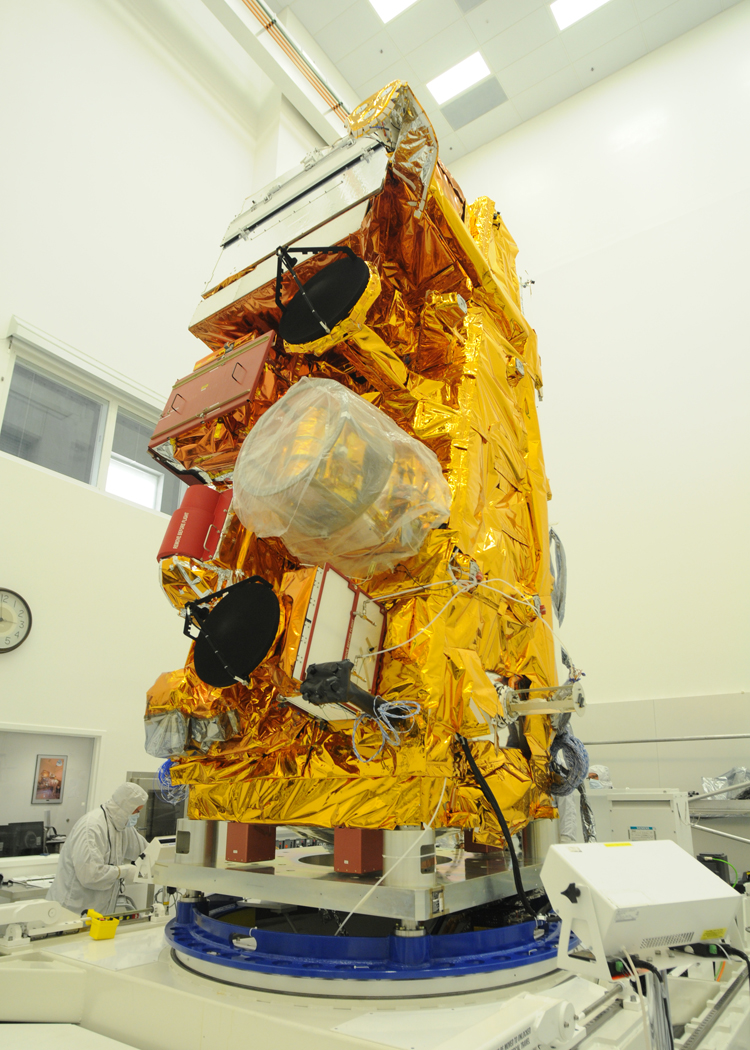
\includegraphics[width=1.2\linewidth]{NPP_satellite_in_cleanroom.jpeg}
        % \caption{Thomas Lumley}
      \end{figure}
    \end{minipage}%
    \hfill%
    \begin{minipage}{0.6\textwidth}\raggedleft
      \begin{itemize}
        \item \textbf{Launch date:} 28 October 2011 at 3:18 pm IST
        \item \textbf{Operator:} 	NASA / NOAA / DoD
        \item \textbf{Period:} 14 times per day 
        \item \textbf{Instruments:} 
        \begin{enumerate}
          \item Visible Infrared Imaging Radiometer Suite (VIIRS)
          \item Advanced Technology Microwave Sounder (ATMS)
          \item Ozone Mapping and Profiler Suite (OMPS)
          \item Cross-track Infrared Sounder (CrIS)
          \item Clouds and the Earth's Radiant Energy System (CERES)
          
        \end{enumerate}
      \end{itemize}      
    \end{minipage} 
    
  \end{frame}
  
  \begin{frame}{Visible Infrared Imaging Radiometer Suite (VIIRS)}
    \noindent\begin{minipage}{0.273\textwidth}
          \begin{figure}
            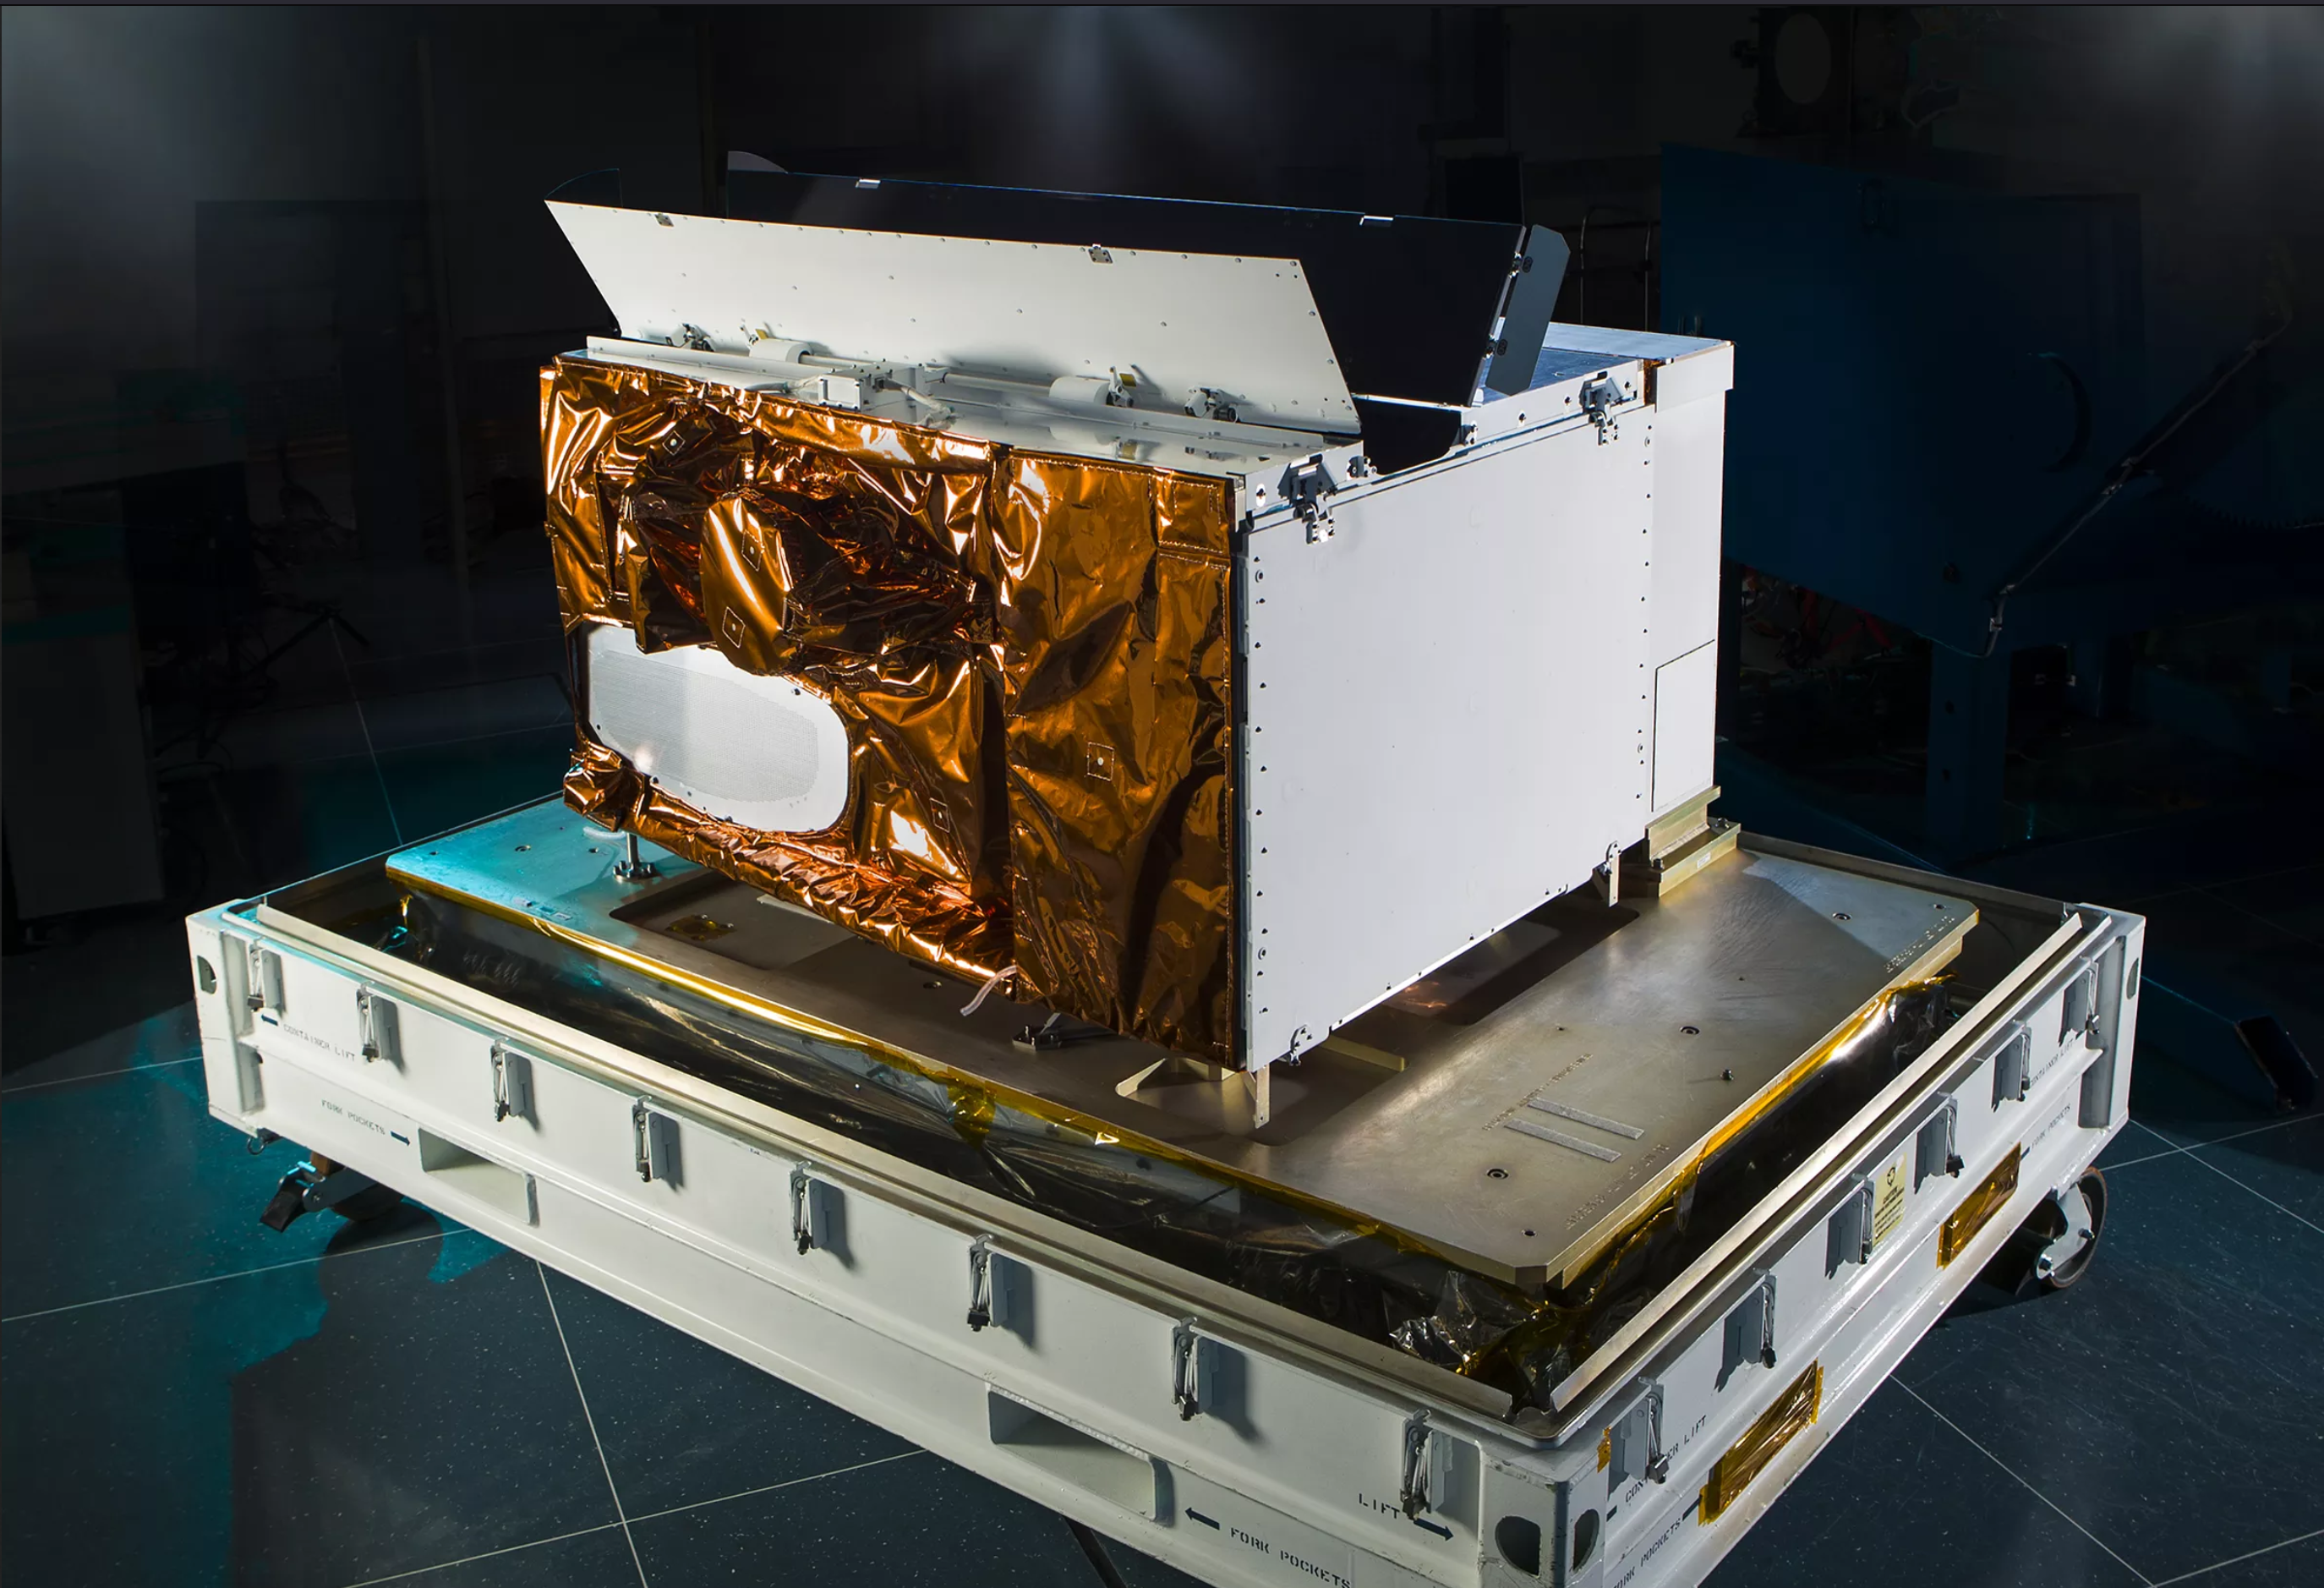
\includegraphics[width=1.45\linewidth]{viirs.png}
          \end{figure}
        \end{minipage}%
        \hfill%
        \begin{minipage}{0.6\textwidth}\raggedleft
          \begin{itemize}
            \item \textbf{No. spectral bands:} 22
            \item \textbf{Uses:} Nighttime lights, fire anomalies, Vegetation Index, etc. 
          \end{itemize}      
        \end{minipage} 
      \end{frame}
      
      \subsection{Bands}
      
      \begin{frame}{Bands}
        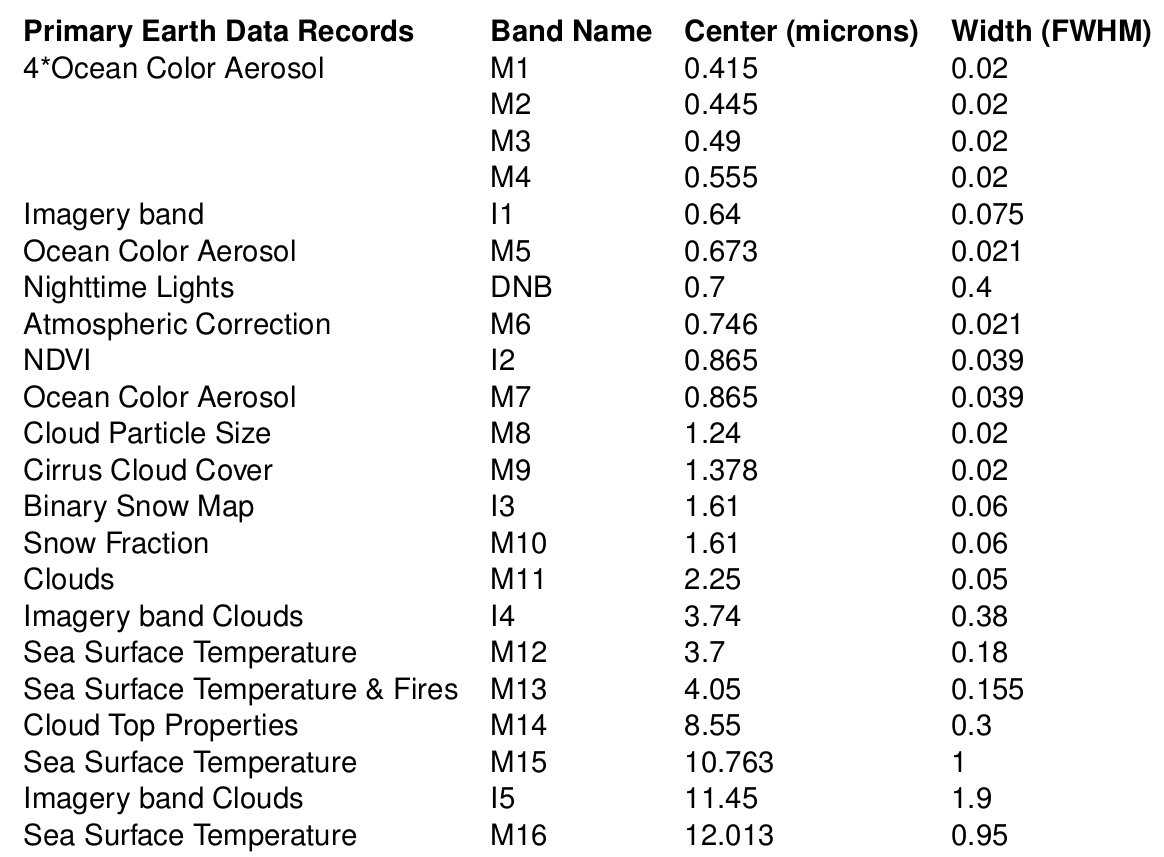
\includegraphics[width = .7\linewidth]{table.png}
        % \scalebox{0.65}{
          %   \begin{tabular}{llll}
  %   \textbf{Primary Earth Data Records}     & \textbf{Band Name} & \textbf{Center (microns)}& \textbf{Width (FWHM)}\\
  %     \multirow{4}{*}{Ocean Color Aerosol}  & M1                 & 0.415                    & 0.02                 \\
  %                                           & M2                 & 0.445                    & 0.02                 \\
  %                                           & M3                 & 0.49                     & 0.02                 \\
  %                                           & M4                 & 0.555                    & 0.02                 \\
  %     Imagery band                          & I1                 & 0.64                     & 0.075                \\
  %     Ocean Color Aerosol                   & M5                 & 0.673                    & 0.021                \\
  %     Nighttime Lights                      & DNB                & 0.7                      & 0.4                  \\
  %     Atmospheric Correction                & M6                 & 0.746                    & 0.021                \\
  %     NDVI                                  & I2                 & 0.865                    & 0.039                \\
  %     Ocean Color Aerosol                   & M7                 & 0.865                    & 0.039                \\
  %     Cloud Particle Size                   & M8                 & 1.24                     & 0.02                 \\
  %     Cirrus Cloud Cover                    & M9                 & 1.378                    & 0.02                 \\
  %     Binary Snow Map                       & I3                 & 1.61                     & 0.06                 \\
  %     Snow Fraction                         & M10                & 1.61                     & 0.06                 \\
  %     Clouds                                & M11                & 2.25                     & 0.05                 \\
  %     Imagery band Clouds                   & I4                 & 3.74                     & 0.38                 \\
  %     Sea Surface Temperature               & M12                & 3.7                      & 0.18                 \\
  %     Sea Surface Temperature \& Fires      & M13                & 4.05                     & 0.155                \\
  %     Cloud Top Properties                  & M14                & 8.55                     & 0.3                  \\
  %     Sea Surface Temperature               & M15                & 10.763                   & 1                    \\
  %     Imagery band Clouds                   & I5                 & 11.45                    & 1.9                  \\
  %     Sea Surface Temperature               & M16                & 12.013                   & 0.95                 \\
  %     \end{tabular}
  % }
\end{frame}

\begin{frame}{Bands}
  \begin{figure}
    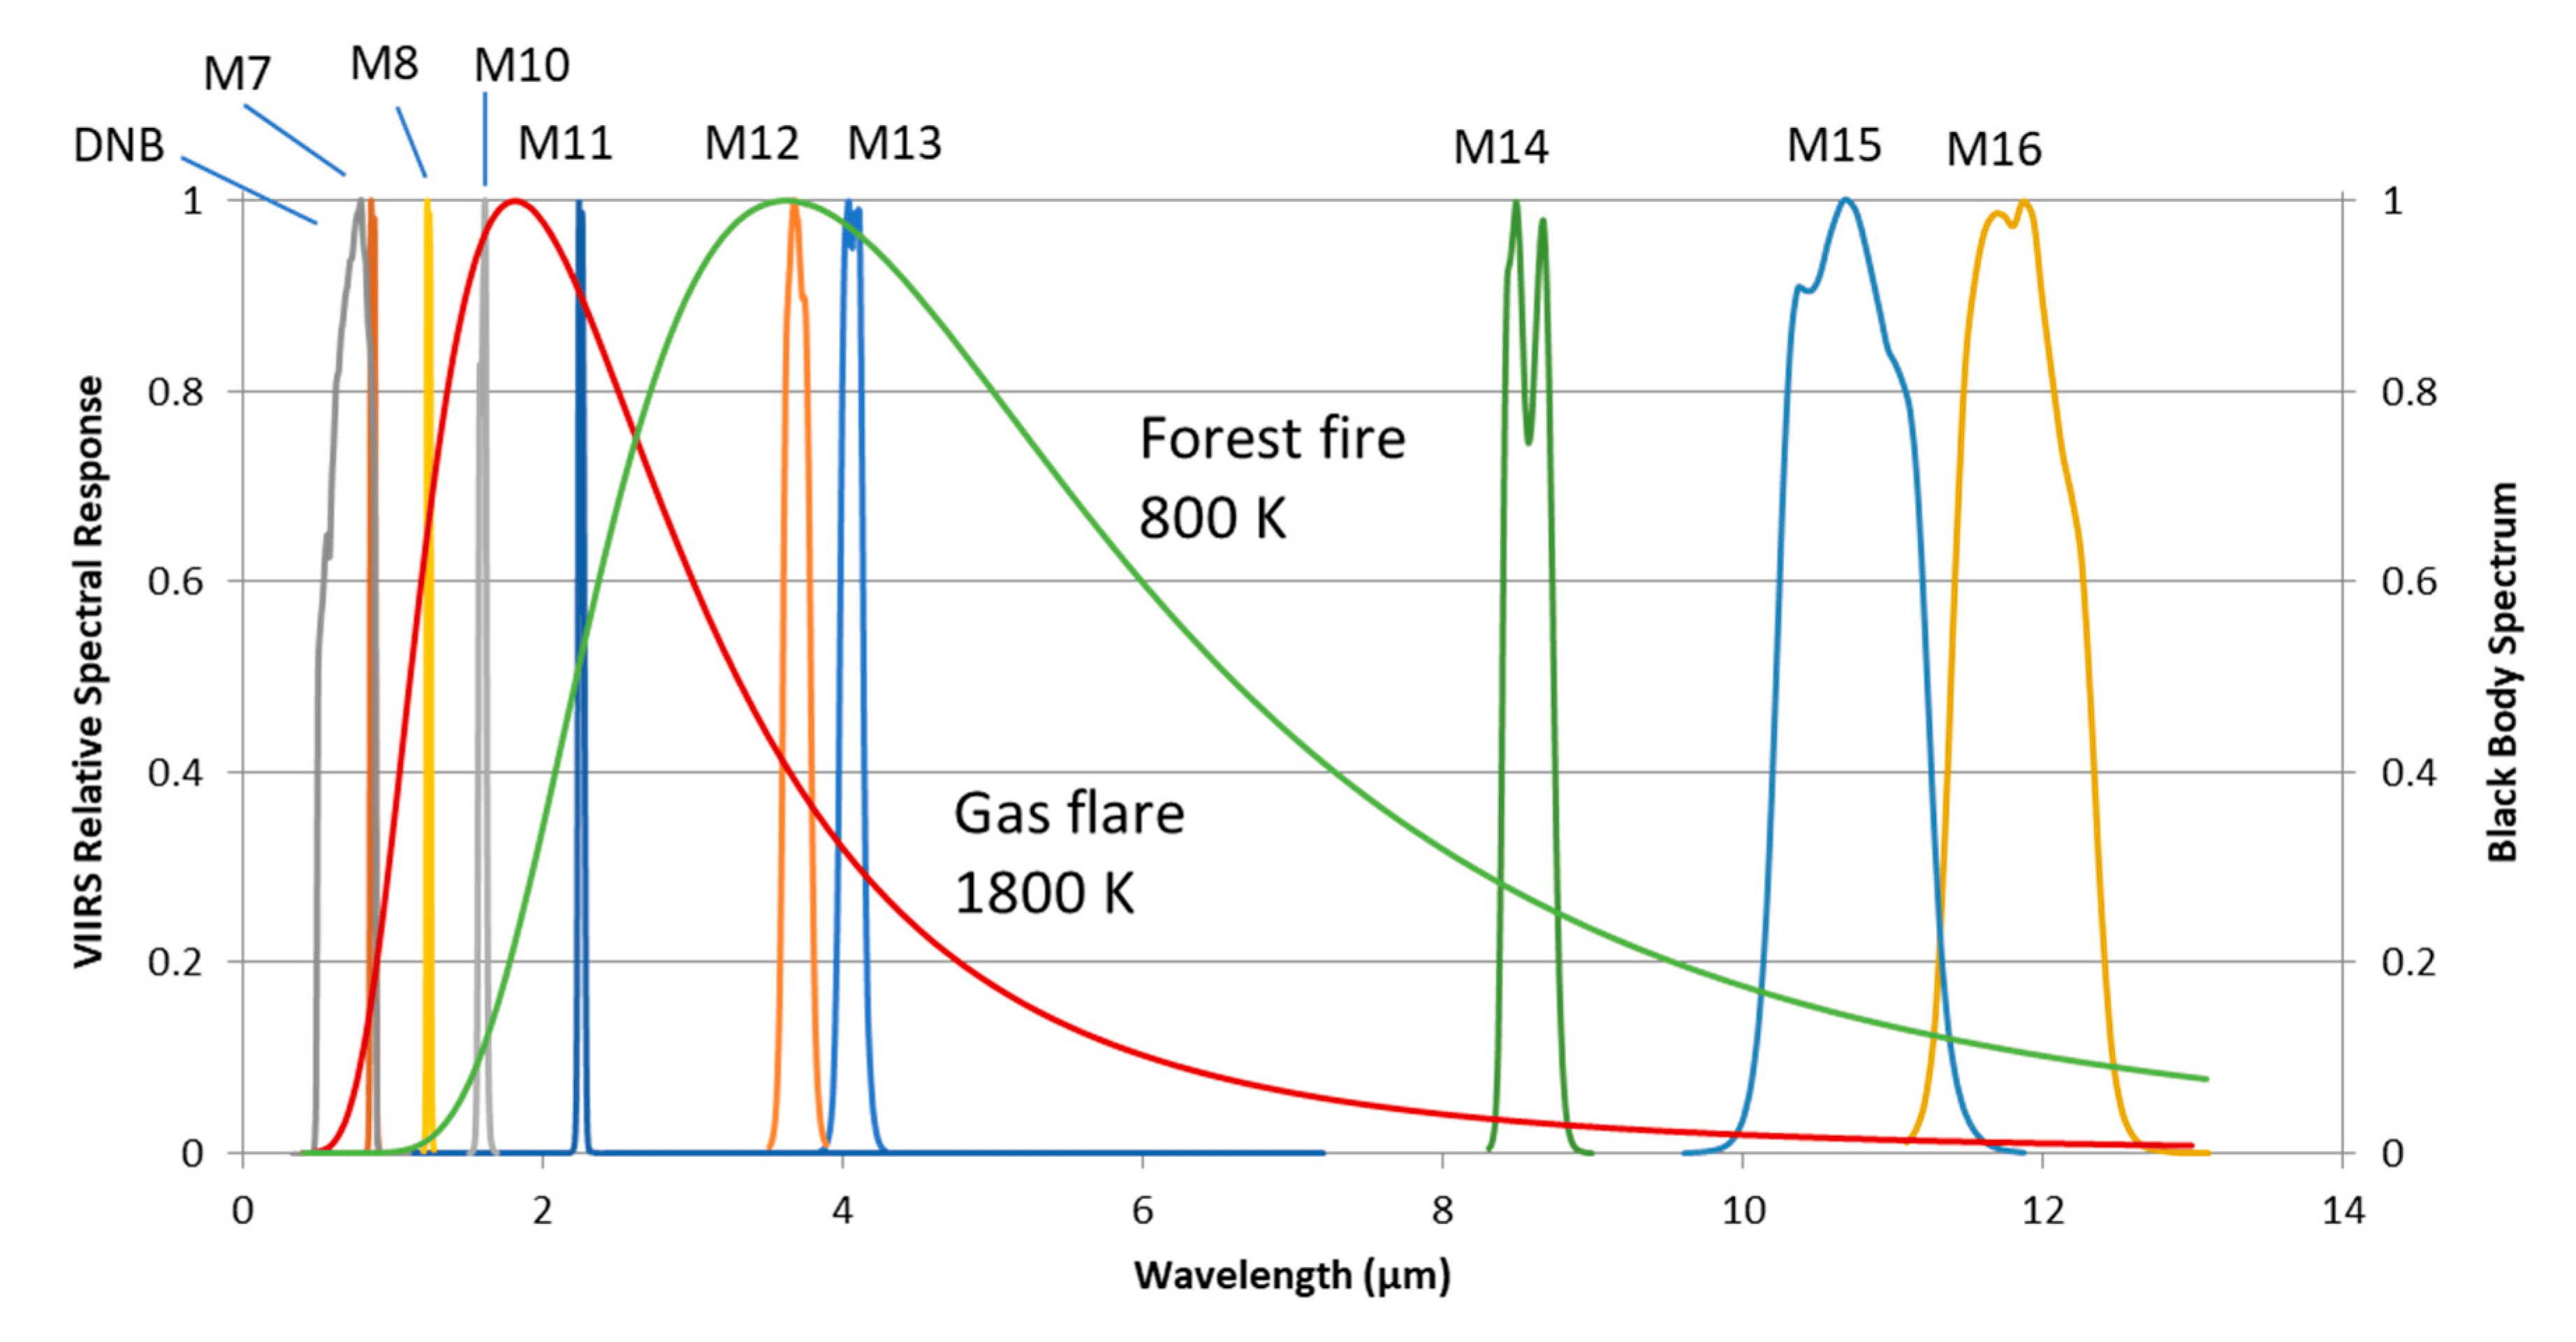
\includegraphics[width=0.75\linewidth]{viirsbands2.png}
    \footfullcite{zhizhinNightTimeDetectionSubpixel2023}
    \footnote{This figure doesn't contain all the 22 VIIRS bands}
  \end{figure}
\end{frame}

\subsection{Applications of VIIRS data}

\begin{frame}{Combining spectral information to generate single band images}
  It is useful to combine the spectral information from the different bands to generate single band images. Each pixel has one value, which makes it easy to utilise them. NOAA often separately releases single band images generated from multiband data. 
  \\
  For example: 
  \begin{enumerate}
    \item Nighttime lights: Radiance measured in \radUnit.  
    \item Active fires: 0 or 1 indicating an active fire at that pixel. 
    \item Vegetation Index: A value between 0 and 1 indicating the amount of vegetation at that pixel.
  \end{enumerate}  
\end{frame}

\begin{frame}{Nighttime lights}{Example 1: January 2021}
  \begin{center}
    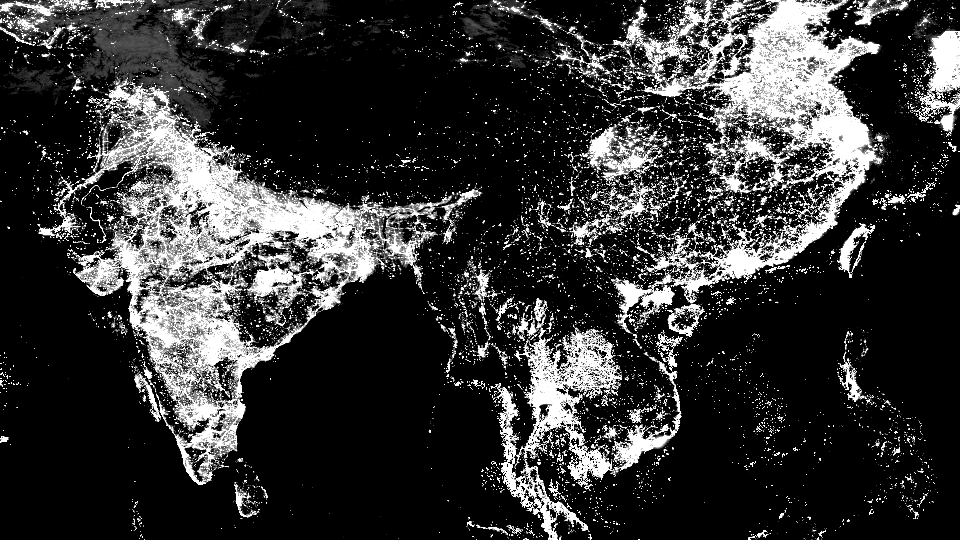
\includegraphics[width = .7\linewidth]{ntl.png}
  \end{center}
\end{frame}

\begin{frame}{Active fires}{Example 2: 1 November 2021}
  \begin{center}
    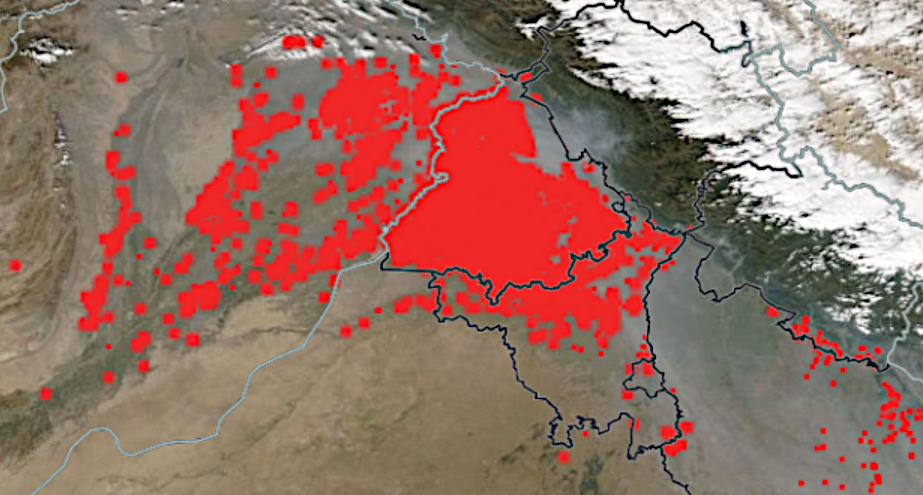
\includegraphics[width = .7\linewidth]{fires.png}
  \end{center}
\end{frame}

\begin{frame}{Enhanced Vegetation Index}{October 2017}
  \begin{center}
    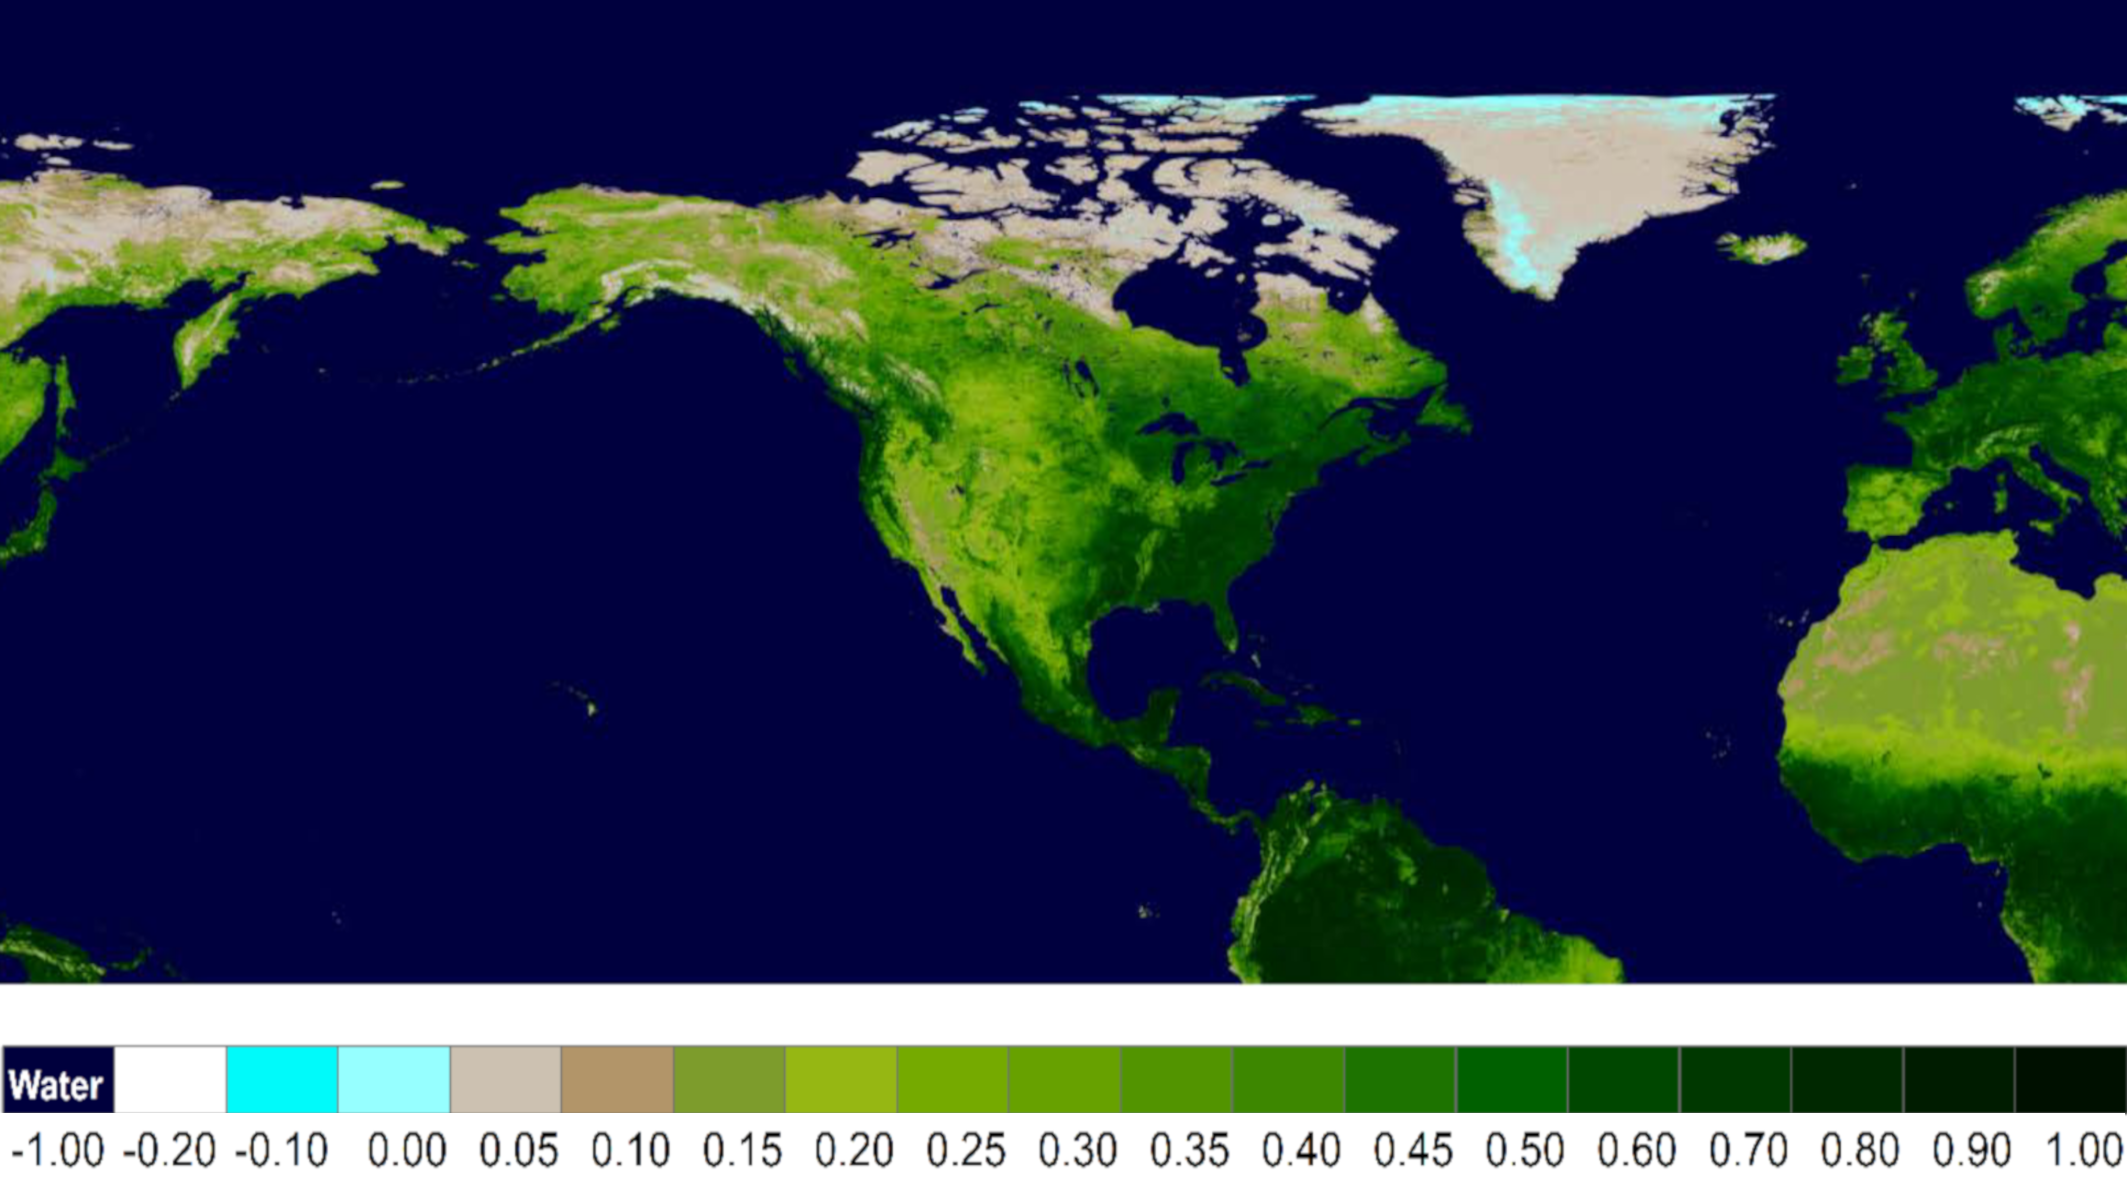
\includegraphics[width = .7\linewidth]{ndvi.png}
  \end{center}
\end{frame}

\subsection{Constructing single band images}

\begin{frame}{Constructing Vegetation Index from spectral information}
  While plants absorb blue light almost completely, they reflect some amount of red and near infrared (NIR) light. 
  Vegetation indices can be created by combining the reflectance measurments at blue, red and NIR \footfullcite{huete2002overview}. NOAA use the following formula for creating Enhanced Vegetation Index from spectral information.
  \begin{equation}
    EVI = 2.5 \frac{\rho_{NIR} - \rho_{red}}{\rho_{NIR} + 6 \rho_{red} - 7.5 \rho_{blue}+ 1}
  \end{equation}
  \\
  \begin{enumerate}
    \item Red:  0.6 - 0.7 ~{\textmu}m
    \item NIR:  0.7 - 1.1 ~{\textmu}m
    \item Blue: 0.44 - 0.5 ~{\textmu}m
  \end{enumerate} 
  This formula was initially used for data from MODIS, but any satellite dataset that contains these bands can be used to construct the EVI. 
  
\end{frame}

\begin{frame}{Bands in VIIRS data for EVI}
  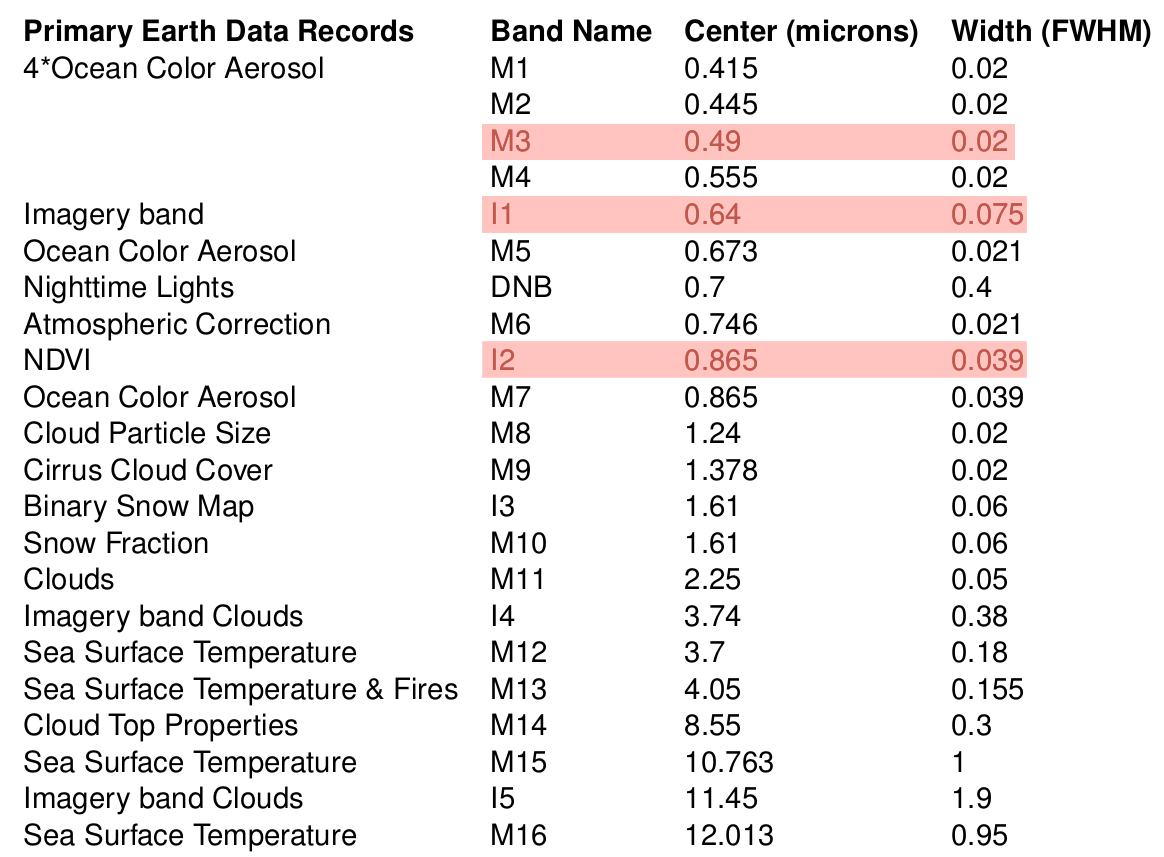
\includegraphics[width = .7\linewidth]{ndvi_bands.png}
\end{frame}

\subsubsection{Extending the framework}

\begin{frame}{Bands in Landsat 9 data for EVI}
  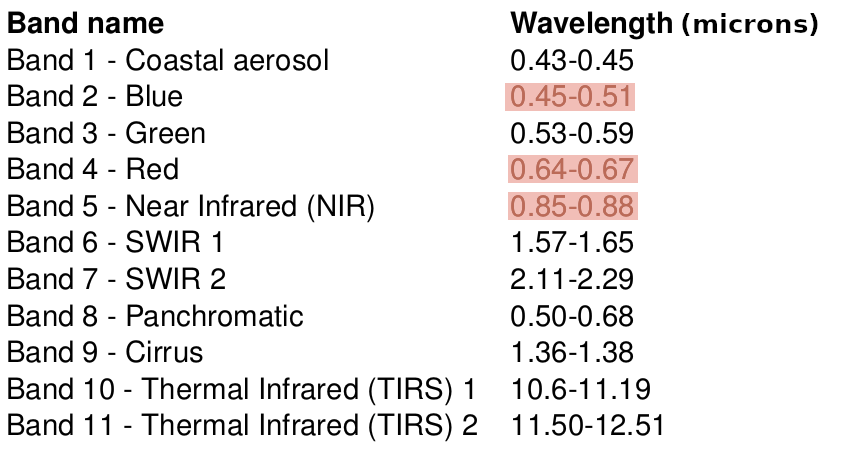
\includegraphics[width = .5\linewidth]{landsat_bands.png}
\end{frame}

\begin{frame}{Bands in Sentinel 2 for EVI}
  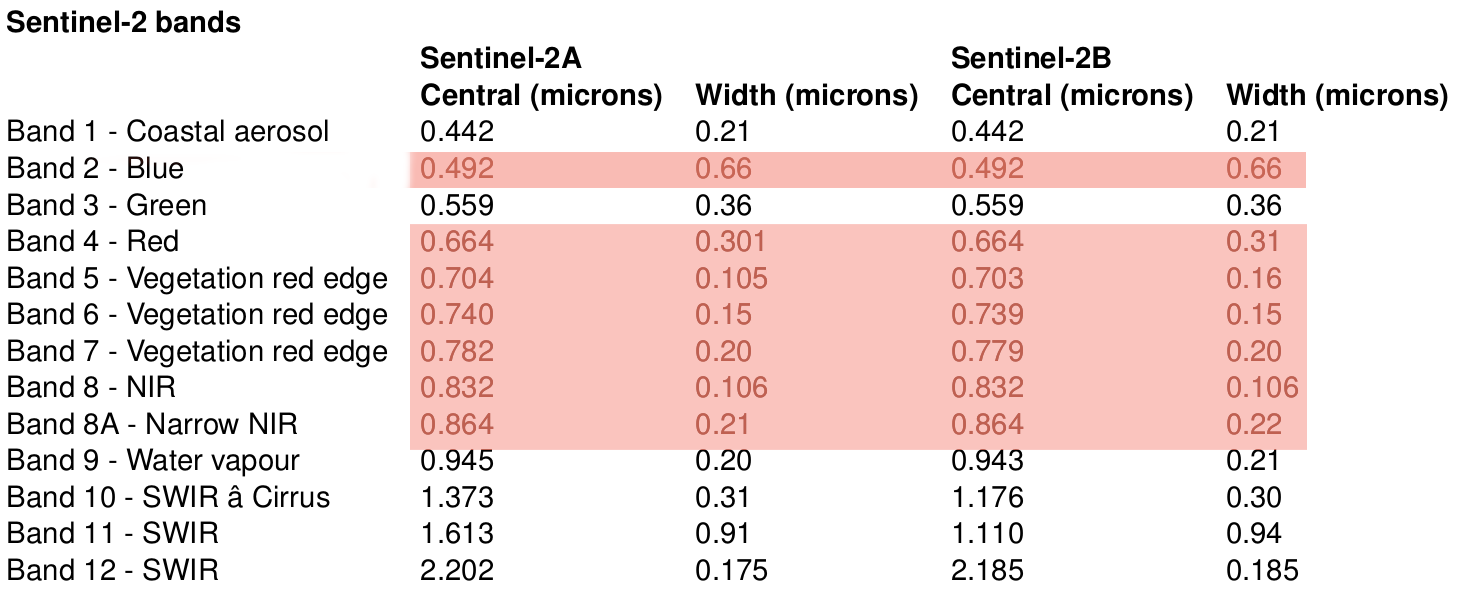
\includegraphics[width = .8\linewidth]{sentinel_evi.png}
  
  %   \scalebox{0.65}{% Please add the following required packages to your document preamble:
  %   % \usepackage{multirow}
  %   \begin{table}[]
    %   \begin{tabular}{lllll}
      % \textbf{Sentinel-2 bands} \\
      
      % & \textbf{Sentinel-2A}      &                                                  & \textbf{Sentinel-2B}                                                        \\
      %                                         & \textbf{Central (microns)} & \textbf{Width (microns)} & \textbf{Central (microns)} &\textbf{Width (microns)} \\
      %   Band 1  - Coastal aerosol                                       & 0.442                                                & 0.21                                          & 0.442                                                & 0.21                                          \\
      %   Band 2  - Blue                                                  & 0.492                                                & 0.66                                          & 0.492                                                & 0.66                                          \\
      %   Band 3  - Green                                                 & 0.559                                                & 0.36                                          & 0.559                                                & 0.36                                          \\
      %   Band 4  - Red                                                   & 0.664                                                &  0.301                                        & 0.664                                                & 0.31                                          \\
      %   Band 5  - Vegetation red edge                                   & 0.704                                                &  0.105                                        & 0.703                                                & 0.16                                          \\
      %   Band 6  - Vegetation red edge                                   & 0.740                                                & 0.15                                          & 0.739                                                & 0.15                                          \\
      %   Band 7  - Vegetation red edge                                   & 0.782                                                & 0.20                                          & 0.779                                                & 0.20                                          \\
      %   Band 8  - NIR                                                   & 0.832                                                & 0.106                                         & 0.832                                                & 0.106                                         \\
      %   Band 8A -  Narrow NIR                                           & 0.864                                                & 0.21                                          & 0.864                                                & 0.22                                          \\
      %   Band 9  - Water vapour                                          & 0.945                                                & 0.20                                          & 0.943                                                & 0.21                                          \\
      %   Band 10 -  SWIR – Cirrus                                        & 1.373                                                & 0.31                                          & 1.176                                               & 0.30                                          \\
      %   Band 11 -  SWIR                                                 & 1.613                                                & 0.91                                          & 1.110                                               & 0.94                                          \\
      %   Band 12 -  SWIR                                                 & 2.202                                                & 0.175                                         & 2.185                                               & 0.185                                        
      %   \end{tabular}
      %   \end{table}}
    \end{frame}

    \subsection{Combining satellite datasets}

    \begin{frame}{Combining satellite datasets}
      Satellite datasets with overlapping bands are often combined to create long timeseries datasets. While one of the most important features of satellite data is high frequency, making long timeseries allow studying long term effects.  
      
    \end{frame}
    
\begin{frame}{Landuse dynamics in Bengaluru}
  \begin{columns}
    \begin{column}{0.45\textwidth}
      \begin{minipage}[c][0.7\textheight][c]{\linewidth}
        \begin{figure}
          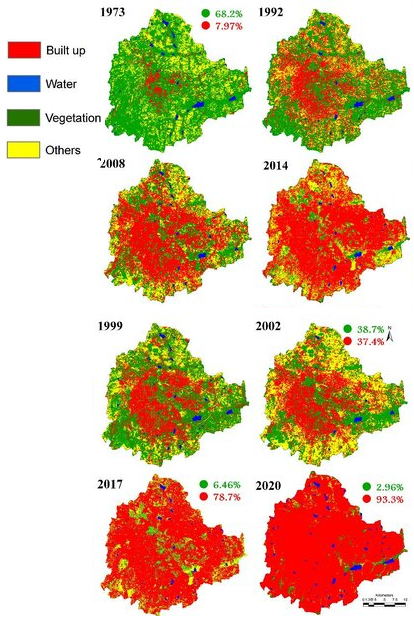
\includegraphics[width=0.75\linewidth]{banglore_vertical.png}
        \end{figure}
      \end{minipage}
    \end{column}
    \begin{column}{0.55\textwidth}
      \begin{minipage}[c][0.6\textheight][c]{\linewidth}
        Two landsat datasets are combined with MODIS to create a long timeseries of landuse of Bengaluru. 
        \begin{itemize}
          \item NIR and MIR bands (bands 3 and 4) of Landsat 1973 data to 23.5 m. 
          \item 3 IR bands of Landsat (band 4-NIR, 5-MIR and 7-MIR) of 1992 to 23.5 m.
          \item 4 IR MODIS bands 2 and 5 to 7 (MOD 09 product) to 250 m.
        \end{itemize}
        \fullcite{ramachandraFrequentFloodsBangalore2017}
      \end{minipage}
    \end{column}
  \end{columns}
\end{frame}

\begin{frame}{Landuse dynamics in Bengaluru}{Previous image shown bigger}
  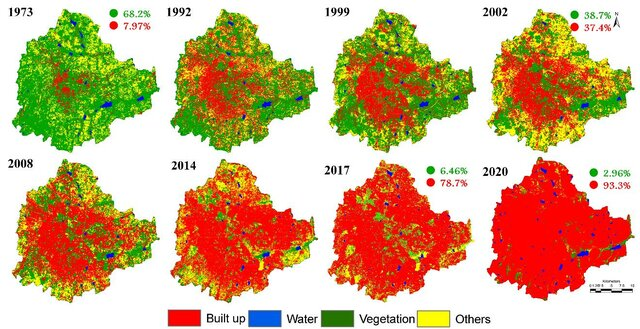
\includegraphics[width=0.9\linewidth]{banglore.jpg}

\end{frame}


\begin{frame}{Harmonized nighttime lights}
  \begin{columns}
    \begin{column}{0.6\textwidth}
      \begin{minipage}[c][0.7\textheight][c]{\linewidth}
        \begin{figure}
          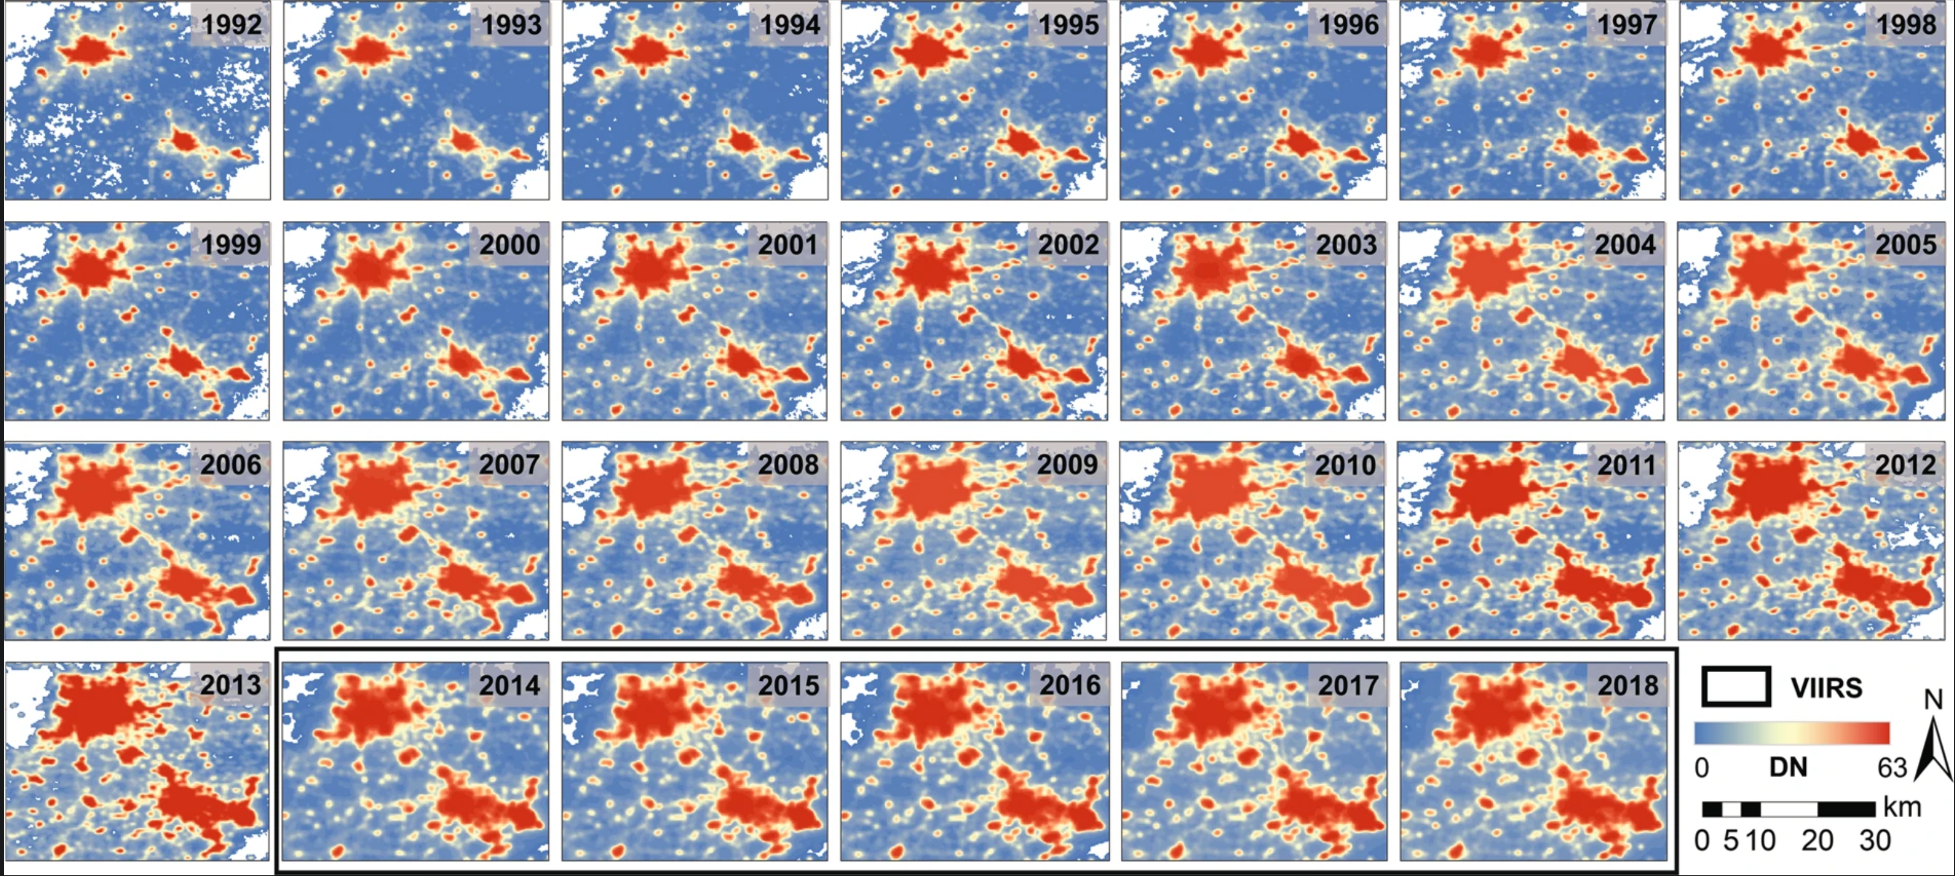
\includegraphics[width=\linewidth]{harmonized.png}
        \end{figure}
      \end{minipage}
    \end{column}
    \begin{column}{0.4\textwidth}
      \begin{minipage}[c][0.6\textheight][c]{\linewidth}
        Combined data from DMSP (1992-2013) with VIIRS(2012-present). 

        \fullcite{liHarmonizedGlobalNighttime2020a}
      \end{minipage}
    \end{column}
  \end{columns}
\end{frame}

\begin{frame}{Harmonized nighttime lights}{Previous image shown bigger}
  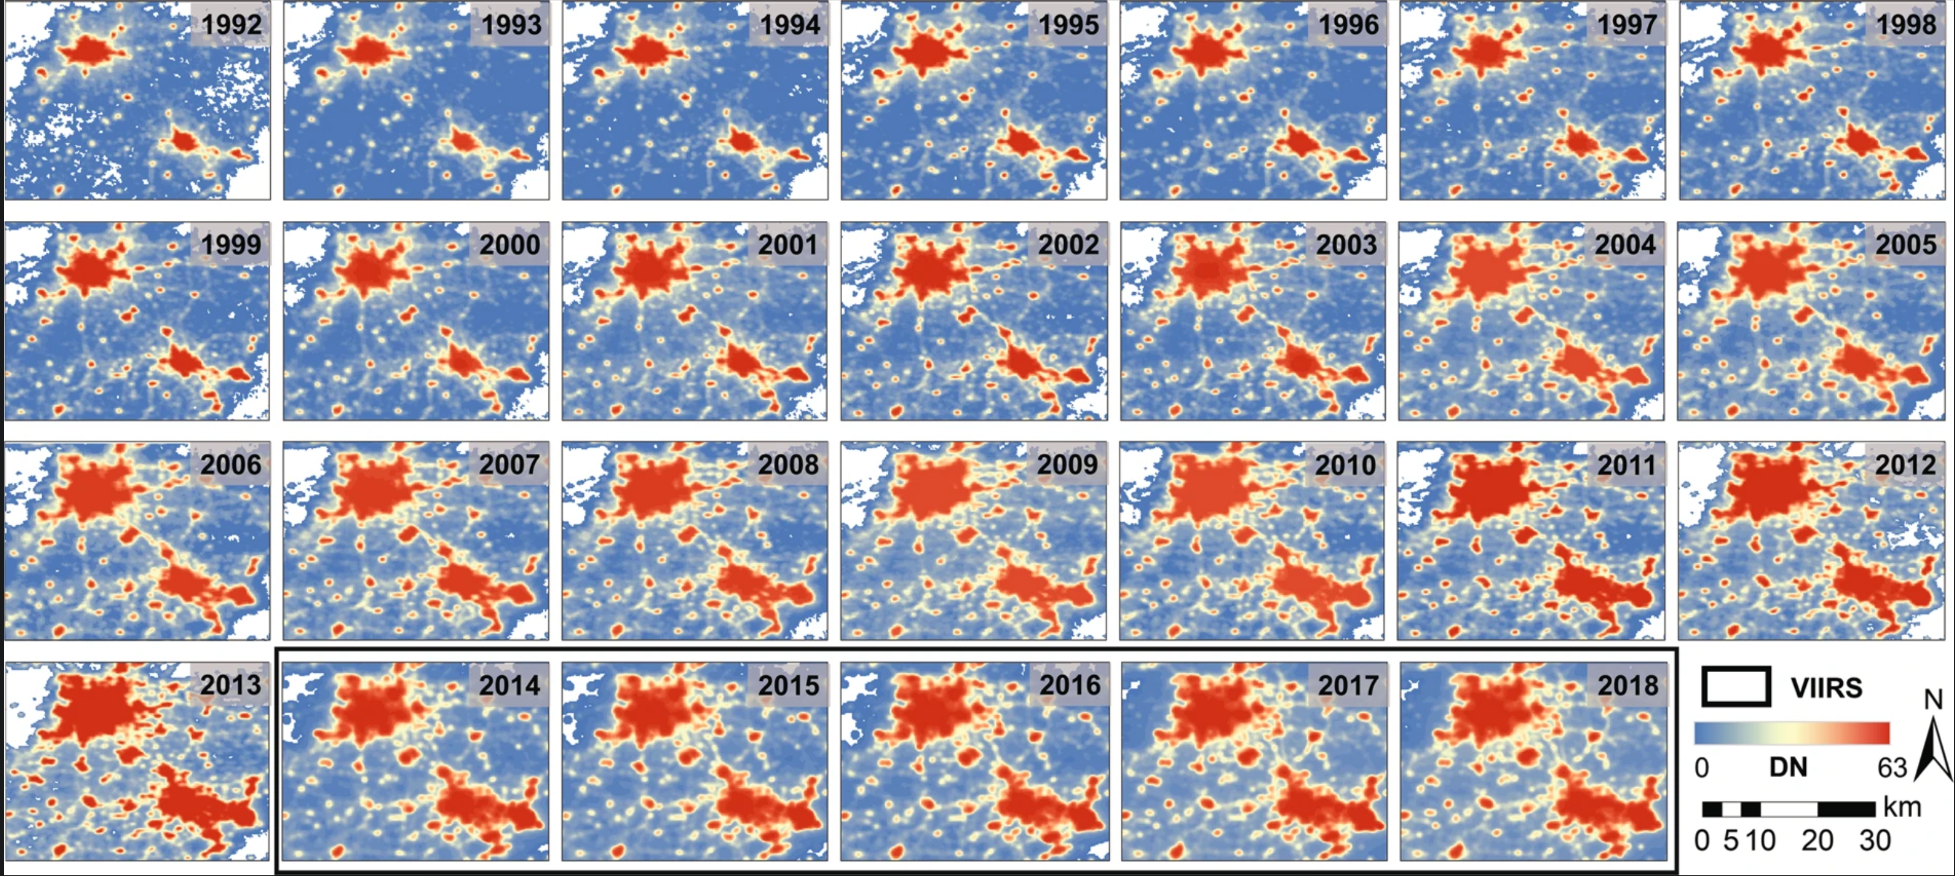
\includegraphics[width=\linewidth]{harmonized.png}
  
\end{frame}
    
    

    \section{Applications}
    \subsection{Crop monitoring}
        \begin{frame}{Crop type mapping using Sentinel-2}
      
      \noindent\begin{minipage}{0.68\textwidth}
        \begin{figure}
          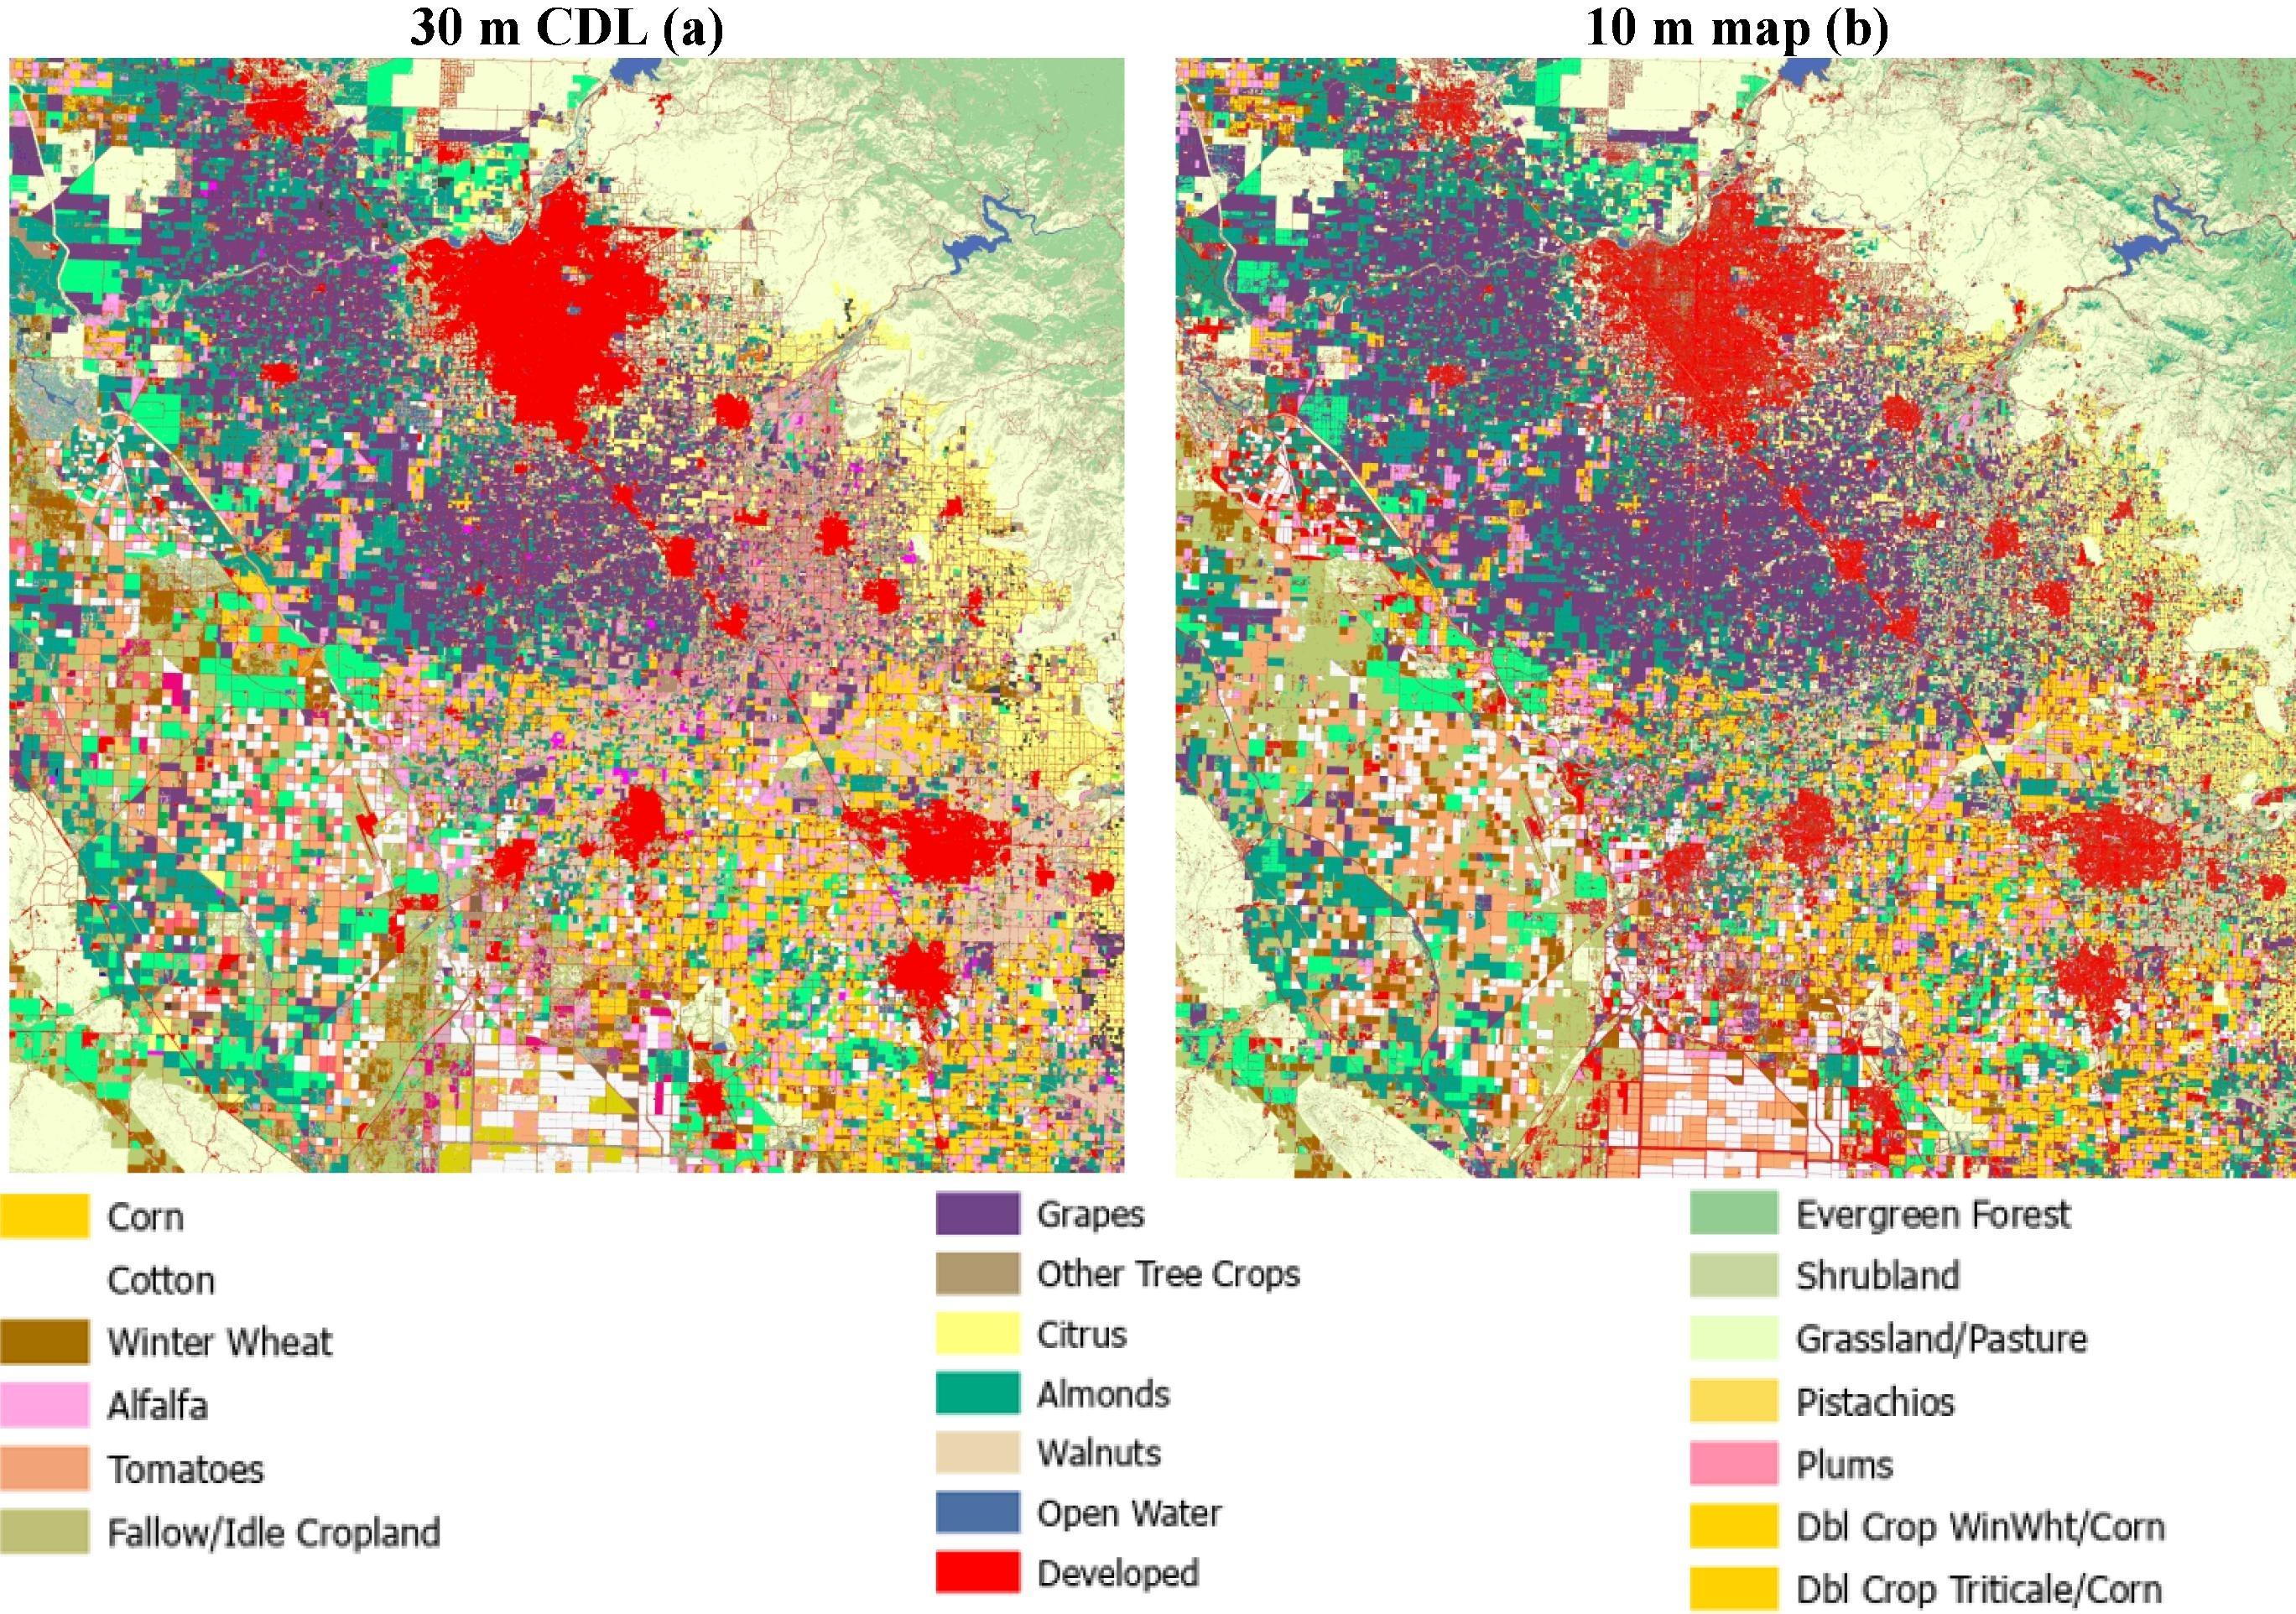
\includegraphics[width = 1\linewidth]{crop.jpg}
        \end{figure}
      \end{minipage}%
      \hfill%
      \begin{minipage}{0.3\textwidth}\raggedright
        Used grouth truth (left) for training a model. 

        \fullcite{tran202210}
      \end{minipage} 
    \end{frame}
    \begin{frame}{Crop health}
      Crop health is estimated using the vegetation index, which was shown earlier. 
      \begin{figure}
        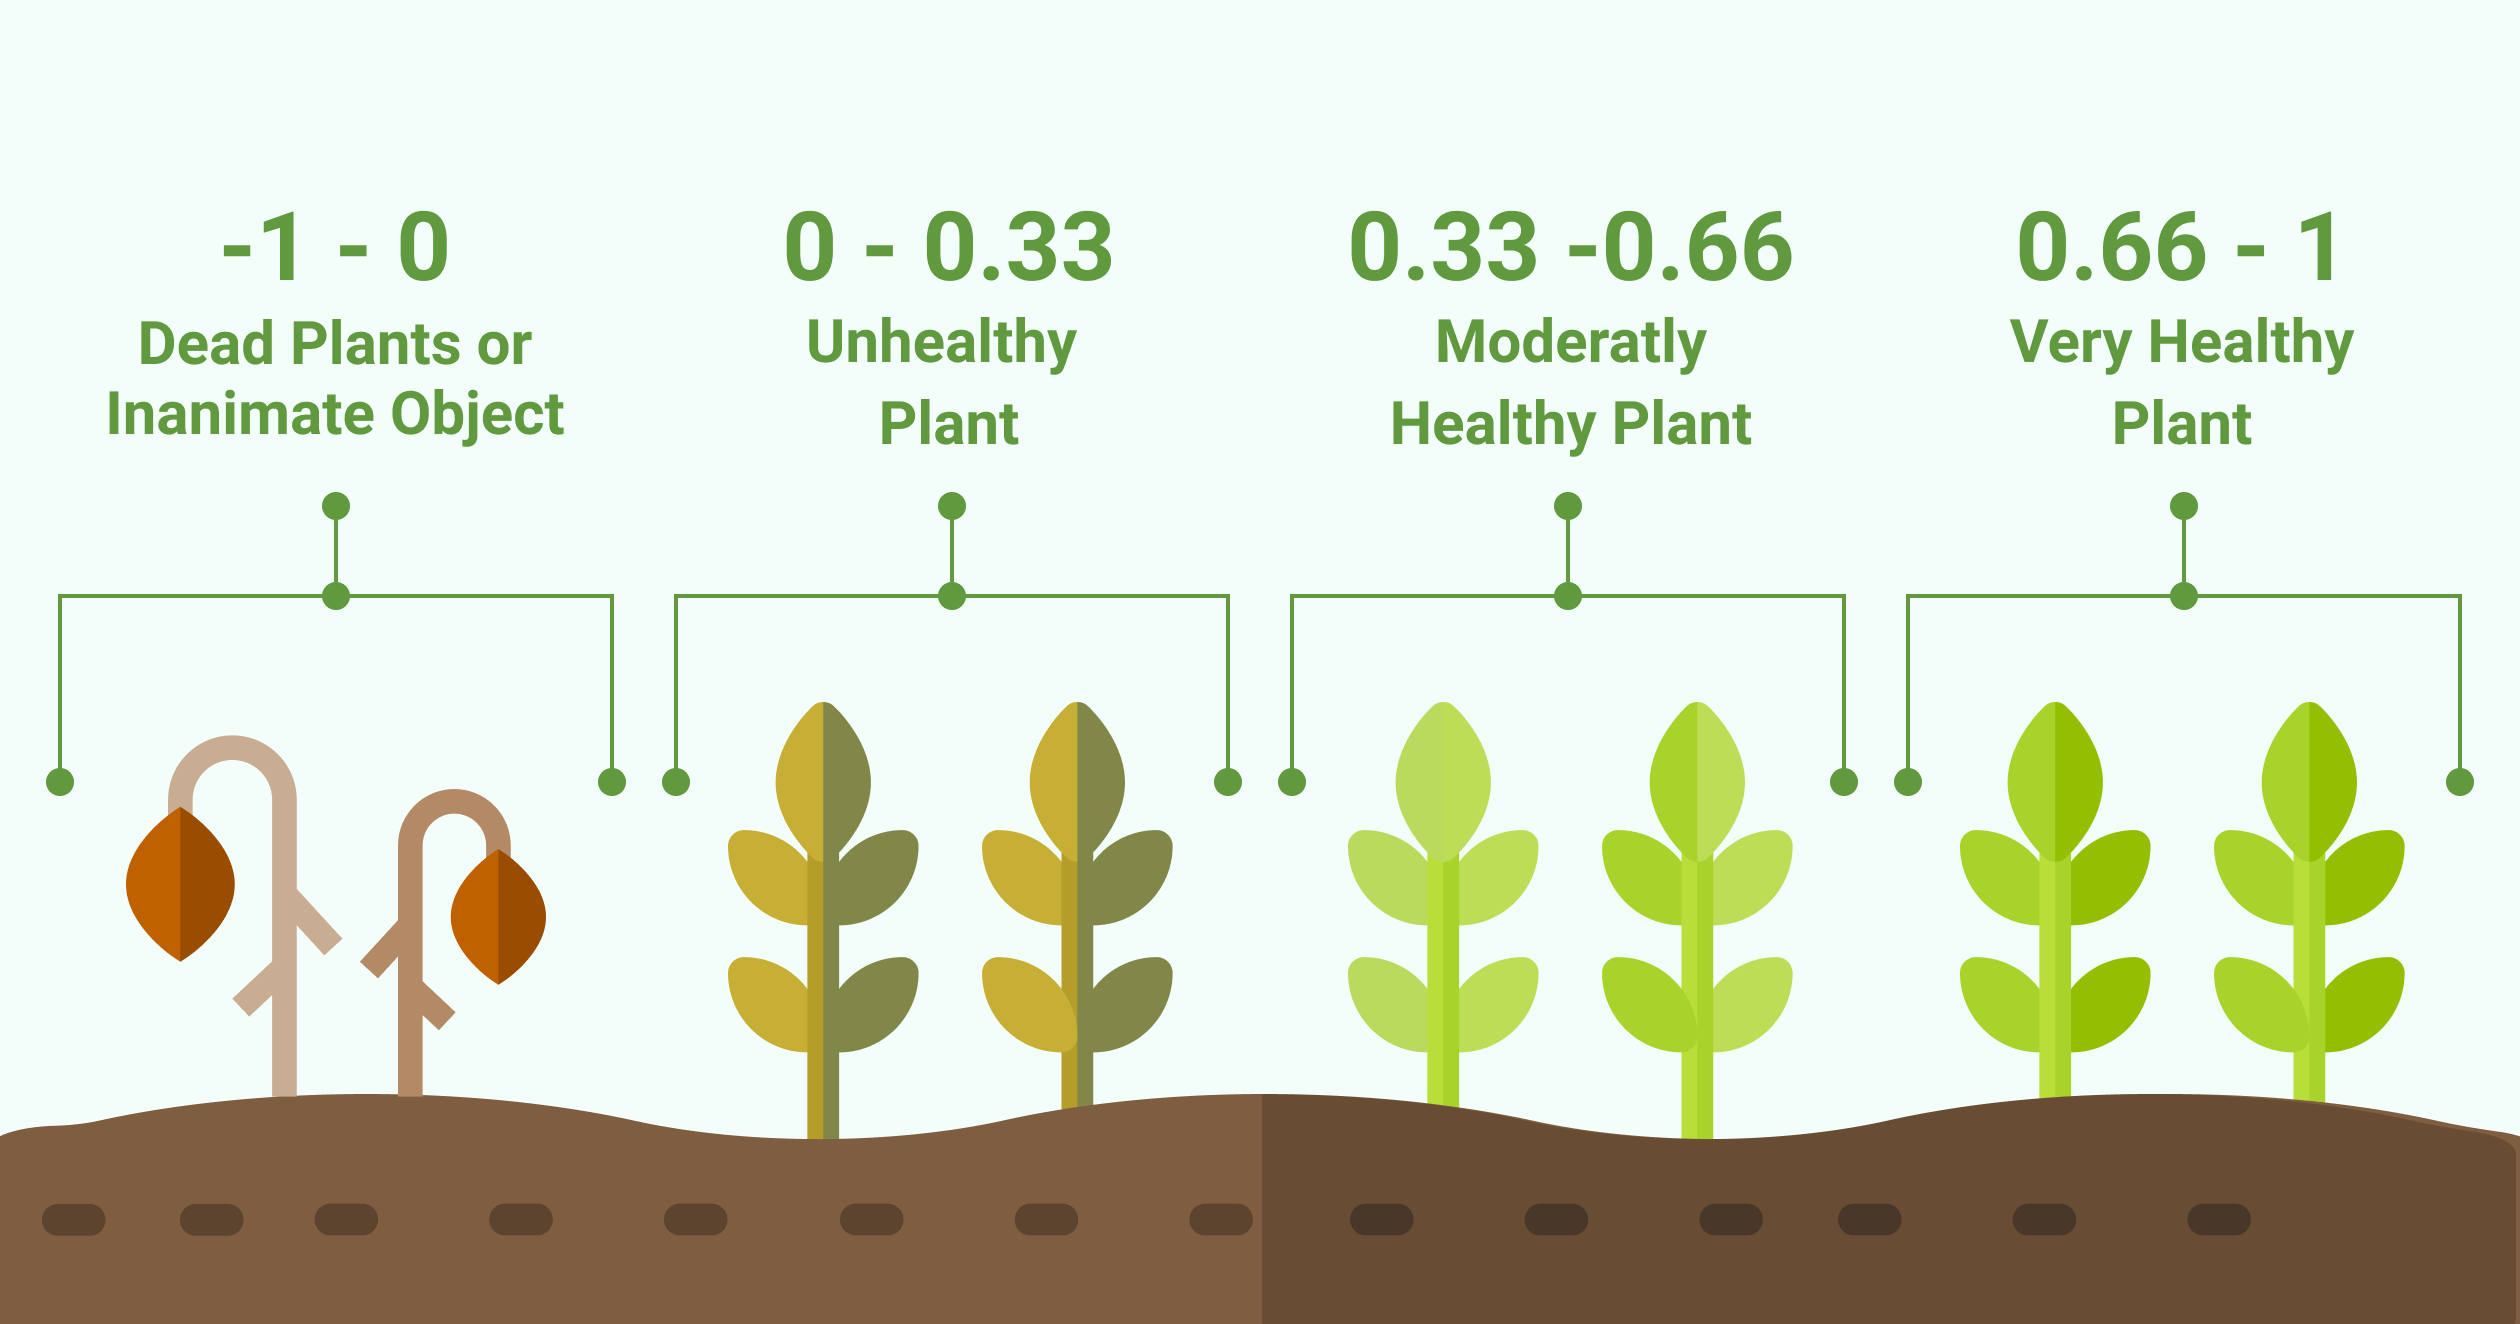
\includegraphics[width = 0.7\linewidth]{plants.png}\footnote{Source: \url{https://phenospex.com/blog/digital-disease-quantification-in-plants-a-tailored-method/plants/}}
      \end{figure}
    \end{frame}

    \begin{frame}{Crop health}
      \begin{figure}
        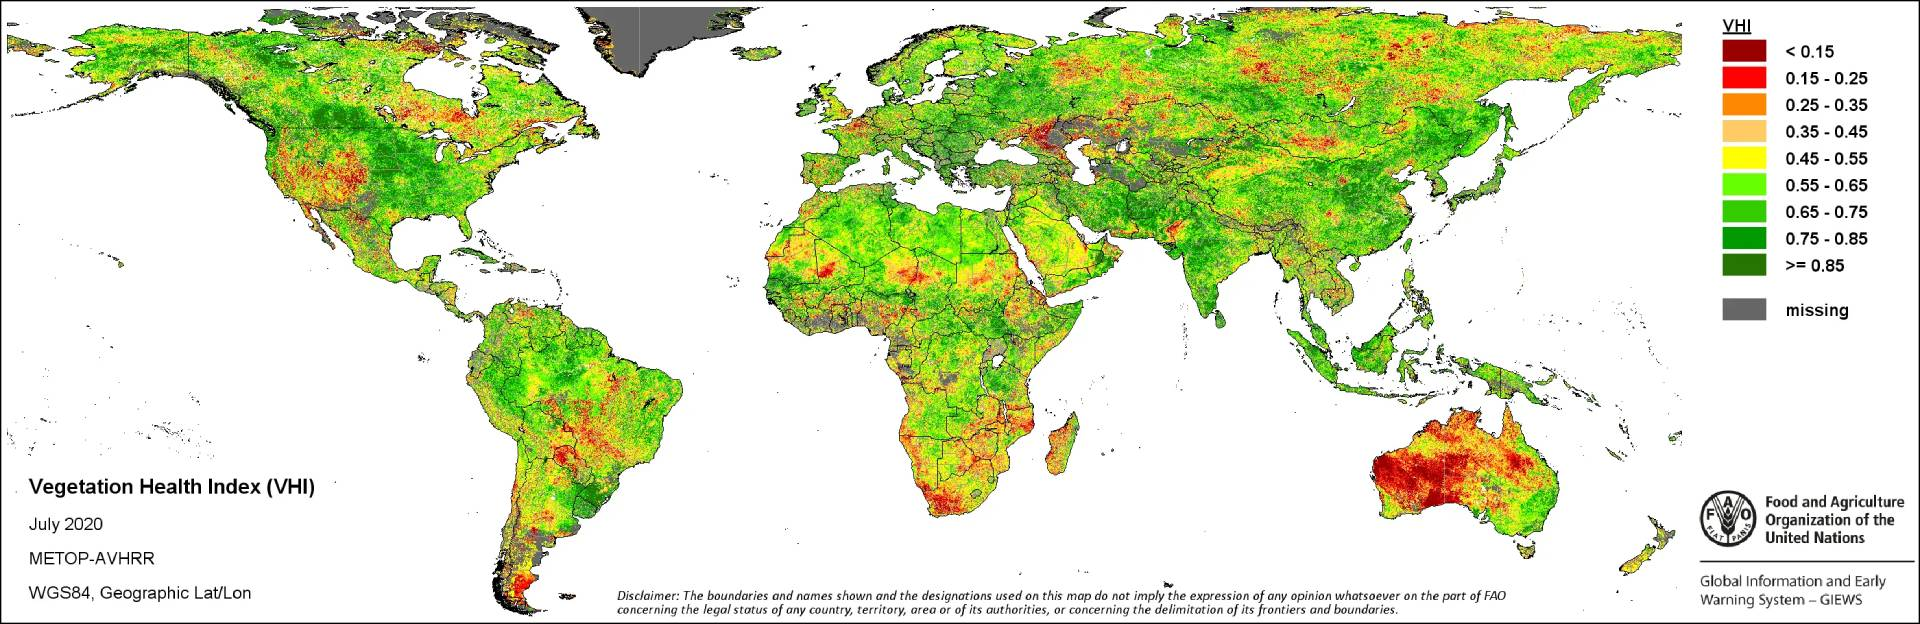
\includegraphics[width = 1\linewidth]{vegetation-health-index.jpg}\footnote{Source: \url{https://data.apps.fao.org/map/catalog/srv/api/records/1eb5883d-05c6-427f-bbf7-8465bfb7069c/attachments/vhi_m.png}}
      \end{figure}
    \end{frame}

  %   \begin{frame}{Applications of satellite imagery}
  %     Satellite imagery has numerous applications across various industries, including:
  
  %     \begin{description}
  %         \item[Agriculture:] Satellite imagery, typically from Sentinel-1, can monitor crop health, identify areas of stress, and optimize irrigation and fertilization practices. 
          
  %         Example: \href{https://www.cropin.com/}{Cropin} 
          
  %         \item[Urban Planning:] Urban planners use satellite imagery to assess land use patterns, monitor urban growth, and plan infrastructure development.
          
  %         \item[Natural Resource Management:] Satellite imagery aids in monitoring deforestation, tracking changes in land cover, and managing water resources.
  %     \end{description}
  % \end{frame}

  % \begin{frame}{Applications of satellite imagery}{Continued}
  %   \begin{description}
  %     \item[Disaster Management:] Satellite imagery provides real-time information during natural disasters, assisting in damage assessment, search and rescue operations, and recovery planning.
          
  %     \item[Logistics and Supply Chain:] Satellite imagery helps optimize logistics routes, monitor transportation networks, and track the movement of goods across regions.
      
  %     \item[Energy:] The energy sector uses satellite imagery for site selection, monitoring infrastructure, and assessing environmental impact.
      
  %     \item[Finance:] Financial institutions leverage satellite imagery for assessing the performance of assets, monitoring economic activity, and evaluating investment opportunities. 
  %   \end{description}
  % \end{frame}
    
    % \begin{frame}{Cropin}
    %   % https://www.cropin.com/blogs/vegetation-index-for-precision-agriculture
    %   % https://www.cropin.com/hubfs/Space4Good%20Case%20study%20June.pdf
    % \end{frame}
    
    \subsection{Fisheries}


    \begin{frame}{Numer8's OFish}{Introduction}
      Numer8's OFish is a mobile application designed to help small-scale fishers navigate the ocean more efficiently and sustainably. 

      It uses the Sentinel data to understand ocean conditions and predict potential fish locations using the following information: 
      
          \begin{itemize}
              \item Sea surface temperature
              \item Ocean currents
              \item Chlorophyll concentration
          \end{itemize}
    \end{frame}
    
    \begin{frame}{Numer8's OFish}{Benefits}
      By combining this data with other factors like historical catch data and user-reported locations, OFish helps fishers to:
      
      \begin{itemize}
          \item Locate potential fishing zones
          \item Navigate safely by providing information on weather hazards
          \item Fish sustainably by targeting specific areas with higher fish concentrations
      \end{itemize}
      
      OFish also offers a complementary system for government authorities, enabling them to:
      
      \begin{itemize}
          \item Monitor fishing activity to combat illegal, unreported, and unregulated (IUU) fishing
          \item Improve fisheries management by understanding where and how fishing is taking place
      \end{itemize}
      
    \end{frame}
        
        \section{Working with satellite data}
        
        \begin{frame}{Image as digits}
        
        \begin{figure}
          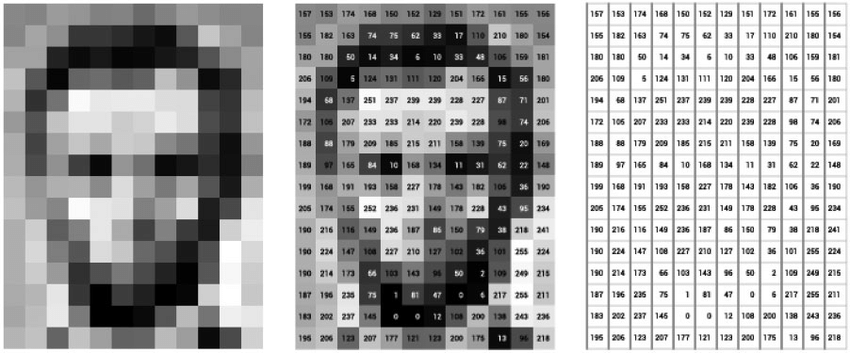
\includegraphics[width=1\linewidth]{image_matrix.png}
        \end{figure}
        \end{frame}
        
        
        \begin{frame}[fragile]
        \frametitle{Satellite image as digits}
        \small
        \begin{verbatim}
48x101 Raster{Float32,2} unnamed with dimensions:
X Mapped{Float32} Float32[72.783335, 72.7875, ..., 72.975, 72.979164] EPSG,
Y Mapped{Float32} Float32[19.266666, 19.2625, ..., 18.854166, 18.85] EPSG
and reference dimensions:
Ti Sampled{DateTime} DateTime[DateTime("2012-12-01T00:00:00")]
extent: Extent(X = (72.78125, 72.98125), Y = (18.847916, 19.26875))
crs: EPSG:4326
mappedcrs: EPSG:4326
parent:
        19.2667  19.2625  19.2583  ..  18.8625  18.8583  18.8542  18.85
72.7833   1.52     0.84     0.64        0.09     0.06     0.07     0.06
72.7875   1.63     1.35     0.86        0.08     0.07     0.05     0.06
72.7917   3.3      2.28     1.26        0.09     0.08     0.07     0.11
:                                  :                     :       
72.9708  31.7     37.09    42.36        1.23     1.06     0.97     0.93
72.975   21.98    28.94    38.1         1.19     0.95     0.86     0.94
72.9792  19.52    26.22    28.3         1.35     1.01     0.87     0.8
        \end{verbatim}
        \end{frame}

        \begin{frame}{QGIS Demonstration}
          \begin{figure}
            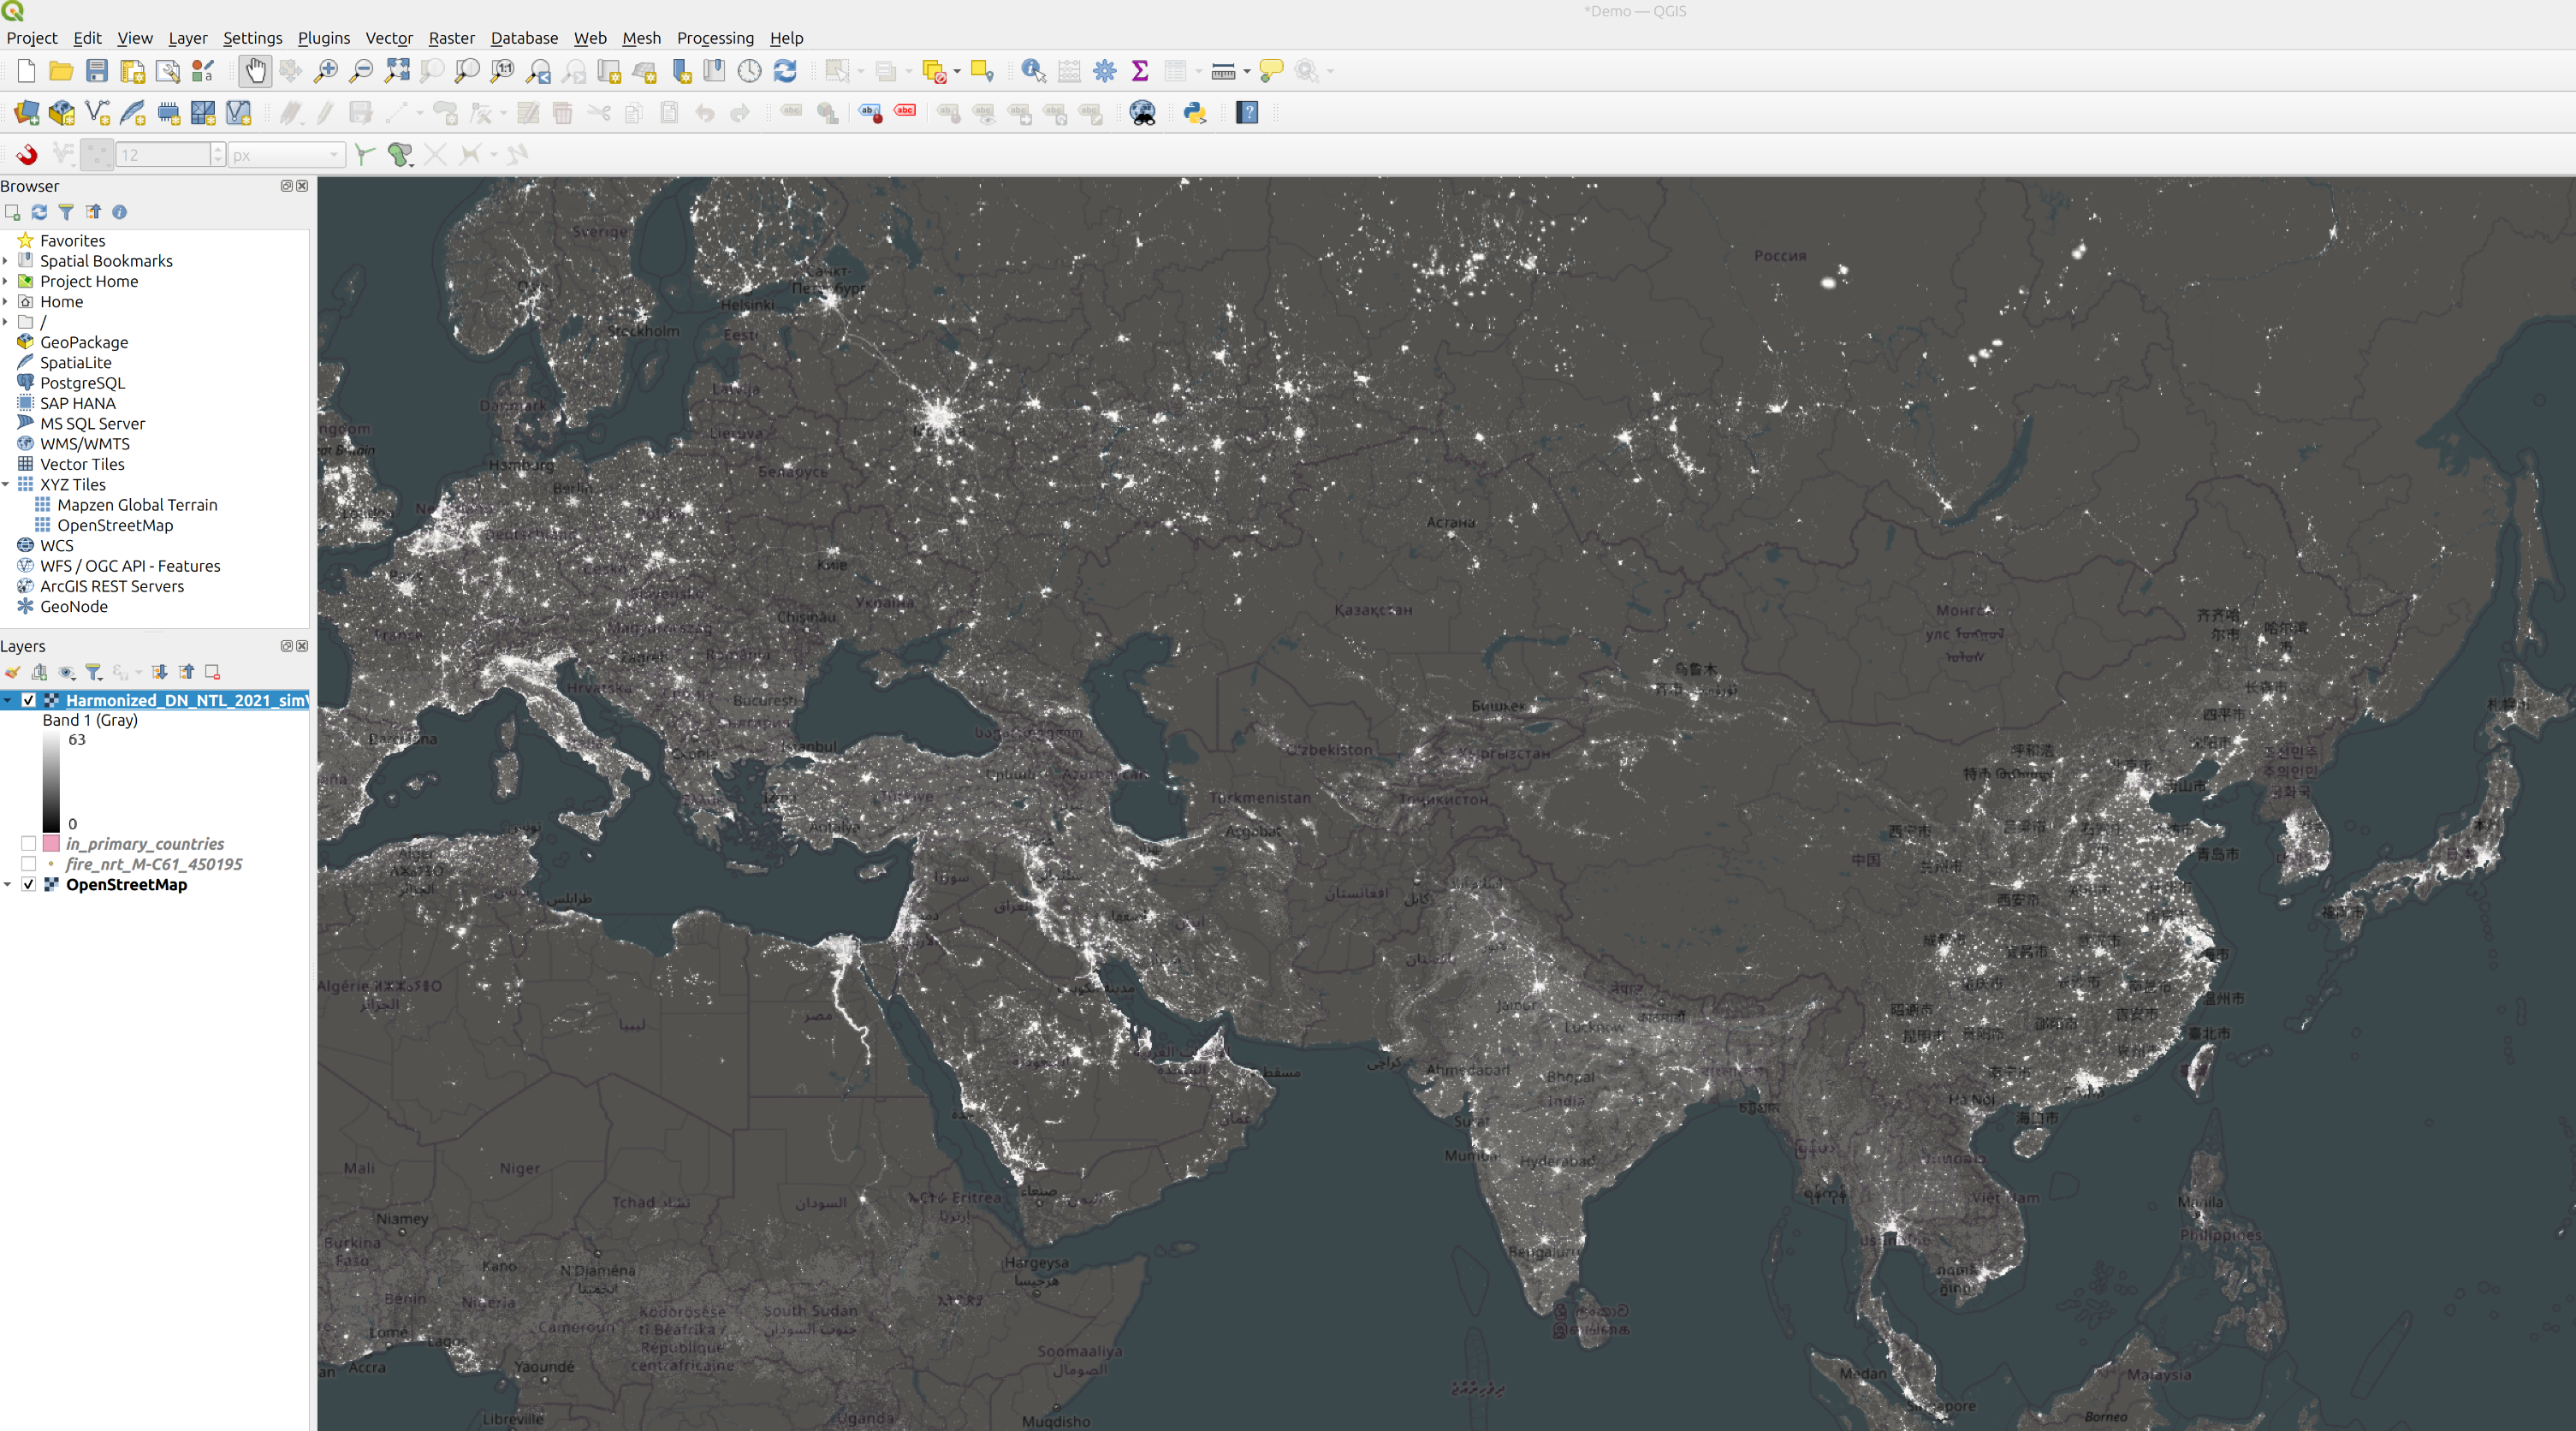
\includegraphics[width=1\linewidth]{qgis.png}
          \end{figure}
        \end{frame}

        \begin{frame}{Raster.jl demonstration}
          \begin{columns}
            \begin{column}{0.6\textwidth}
              \begin{minipage}[c][0.7\textheight][c]{\linewidth}
                \begin{figure}
                  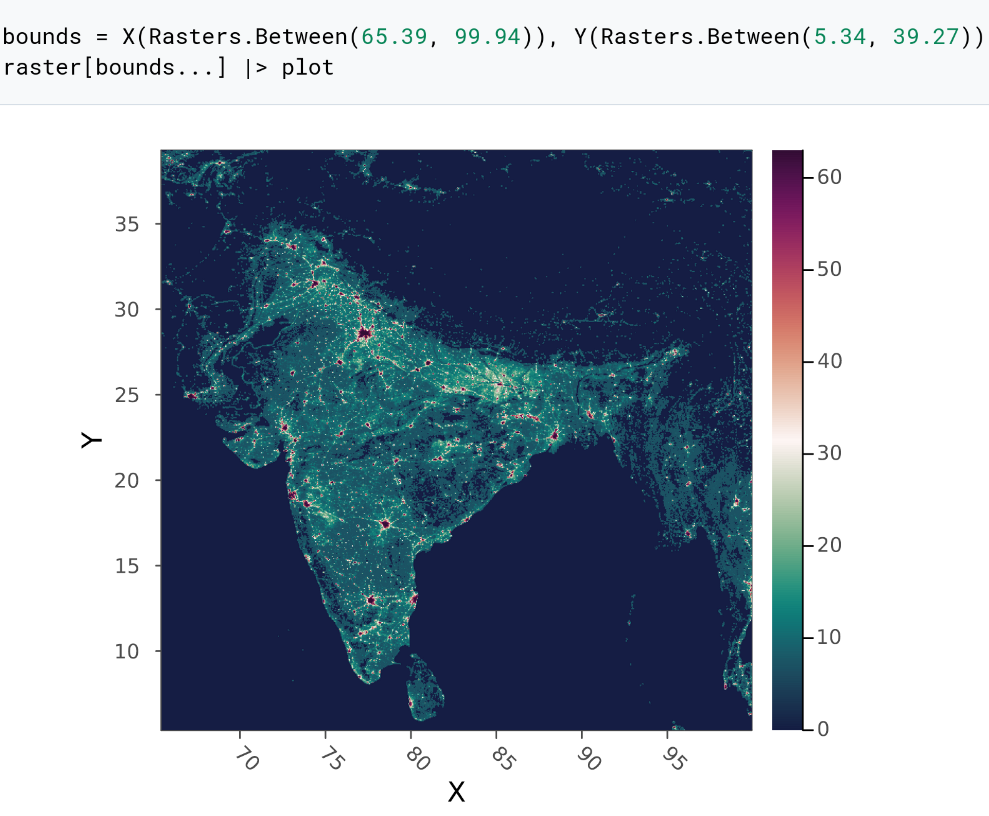
\includegraphics[width=\linewidth]{rasters_demo.png}
                \end{figure}
              \end{minipage}
            \end{column}
            \begin{column}{0.4\textwidth}
              \begin{minipage}[c][0.6\textheight][c]{\linewidth}
                  \url{https://deepnote.com/viewer/github/xKDR/datascience-tutorials/blob/main/rasters.ipynb}
                  \url{https://youtu.be/PqWuGsVQdLw}
              \end{minipage}
            \end{column}
          \end{columns}
        \end{frame}

        \begin{frame}{The effectiveness of Julia}
          \begin{itemize}
            \item All the processes shown can be effectively done using other languages such as Python. 
            \item Julia stands out when it a lot more processing is required, such as processing many images together. 
            \item Rasters.jl allows images to be stacked together, processed efficiently. 
          \end{itemize}
        \end{frame}

        \begin{frame}{The NighttimeLights.jl package}{\url{https://github.com/xKDR/NighttimeLights.jl}}
          \begin{itemize}
            \item The nighttime light package is built on top of Rasters.jl. It provides functions for cleaning the data. 
            \item In some cases, 10s or 100s of images are stacked together, and processing is done for each pixel. 
          \end{itemize}
          \fullcite{patnaik2022foundations}
        \end{frame}

        \begin{frame}{Attenuation-correction process}
          \begin{itemize}
            \item For each pixel in the VIIRS monthly nighttime lights data, we get the radiance of that month and the number of days in the month that weren't cloudy.
            \item We find that months with low number of cloud-free days show lower radiance. 
            \item This attenuation is corrected using a pixel level statistical process. 
          \end{itemize}
            
        \end{frame}

        \begin{frame}{Attenuation of pixel's radiance}
          \begin{figure}
            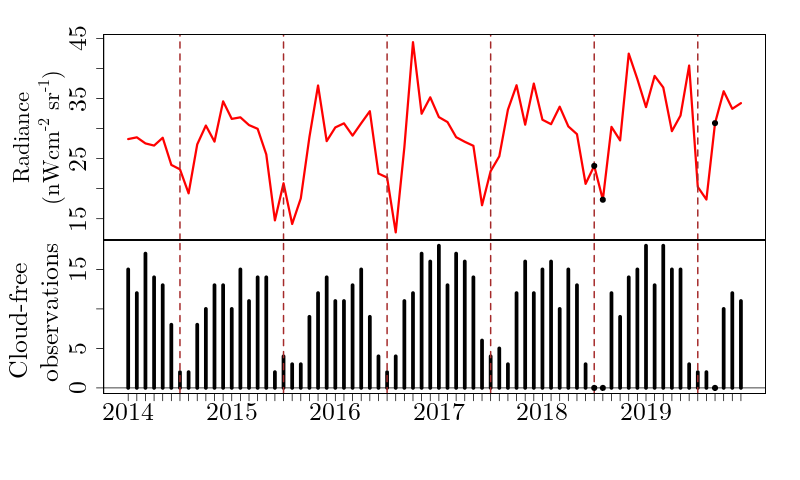
\includegraphics[width=0.8\linewidth]{biased_pixel.png}
          \end{figure}
        \end{frame}

        \begin{frame}{Relationship between radiance and cloudiness}
          \begin{figure}
            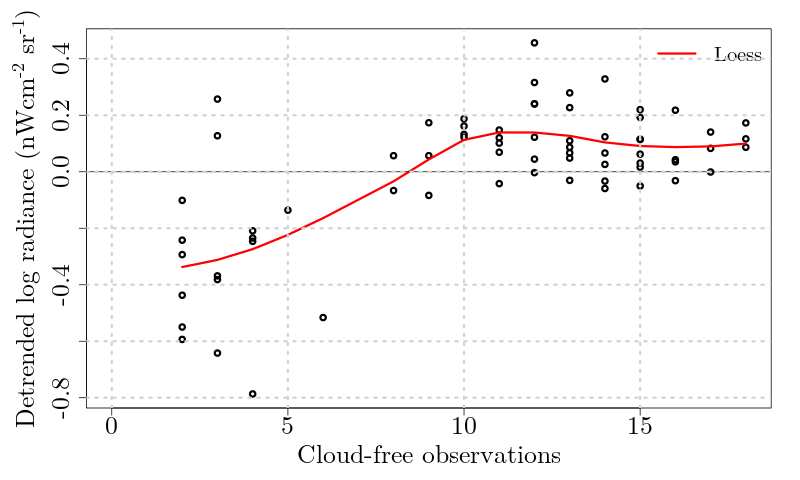
\includegraphics[width=0.8\linewidth]{loess.png}
          \end{figure}
        \end{frame}


        \begin{frame}{Corrected radiance}
          \begin{columns}
            \begin{column}{0.6\textwidth}
              \begin{minipage}[c][0.7\textheight][c]{\linewidth}
                \begin{figure}
                  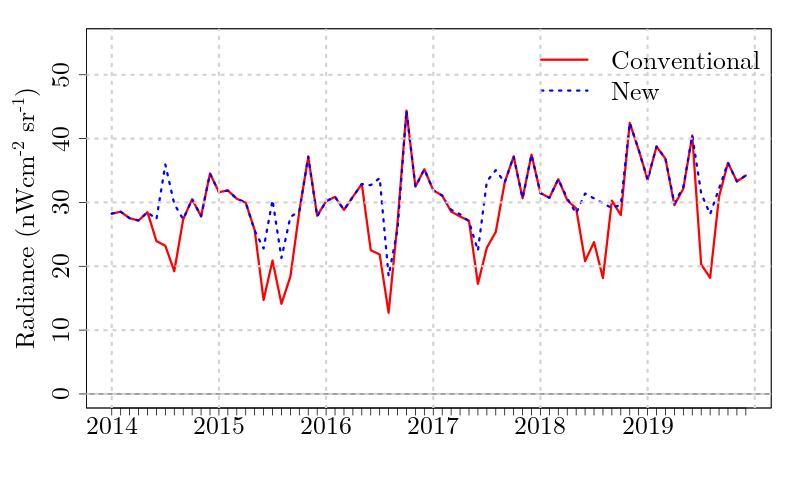
\includegraphics[width=\linewidth]{biasCorrected.png}
                \end{figure}
              \end{minipage}
            \end{column}
            \begin{column}{0.4\textwidth}
              \begin{minipage}[c][0.6\textheight][c]{\linewidth}
                This is done for each pixel in a selected region.
                
                For reference, a bounding box around India contains $\approx$ 50 million pixels. 
                 \\ 
                \fullcite{patnaikCloudsGotMy2021a}
              \end{minipage}
            \end{column}
          \end{columns}
        \end{frame}


        \begin{frame}
          \hfill {\LARGE Thank you}.
          
          \vfill
          \vfill
          
          \hfill \url{https://xkdr.org}
        \end{frame}

        \begin{frame}[allowframebreaks]
          \frametitle{Bibliography}
          \renewcommand*{\bibfont}{\scriptsize}\printbibliography
        \end{frame}
        
\end{document}
